\documentclass[conference]{IEEEtran}
\IEEEoverridecommandlockouts
\usepackage[T1]{fontenc}
\usepackage{cite}
\usepackage{amsmath,amssymb}
\usepackage{graphicx}
\usepackage{booktabs}
\usepackage{multirow}
\usepackage{xcolor}
\usepackage{url}
\usepackage{tikz}
\usetikzlibrary{arrows.meta,positioning}
\usepackage[hidelinks]{hyperref}
\def\UrlBreaks{\do\/\do-\do.\do_}

% generated by experiments/paper_numbers.py from results/summary.json -- do not edit
\makeatletter
\newcommand{\R}[1]{\ifcsname R@#1\endcsname\csname R@#1\endcsname\else\textbf{??\detokenize{#1}}\fi}
\expandafter\def\csname R@abl.dafny.fullsystem.correct\endcsname{68.0}
\expandafter\def\csname R@abl.dafny.fullsystem.delta\endcsname{+0.0}
\expandafter\def\csname R@abl.dafny.fullsystem.sd\endcsname{2.7}
\expandafter\def\csname R@abl.dafny.no_dev_fixes.correct\endcsname{61.5}
\expandafter\def\csname R@abl.dafny.no_dev_fixes.delta\endcsname{-6.5}
\expandafter\def\csname R@abl.dafny.no_dev_fixes.falsesuccess\endcsname{0.0}
\expandafter\def\csname R@abl.dafny.no_dev_fixes.hi\endcsname{-2.6}
\expandafter\def\csname R@abl.dafny.no_dev_fixes.intact\endcsname{100.0}
\expandafter\def\csname R@abl.dafny.no_dev_fixes.lo\endcsname{-10.8}
\expandafter\def\csname R@abl.dafny.no_dev_fixes.p\endcsname{= 0.011}
\expandafter\def\csname R@abl.dafny.no_dev_fixes.sd\endcsname{1.5}
\expandafter\def\csname R@abl.dafny.no_guard.correct\endcsname{68.0}
\expandafter\def\csname R@abl.dafny.no_guard.delta\endcsname{+0.0}
\expandafter\def\csname R@abl.dafny.no_guard.falsesuccess\endcsname{0.0}
\expandafter\def\csname R@abl.dafny.no_guard.hi\endcsname{+0.0}
\expandafter\def\csname R@abl.dafny.no_guard.intact\endcsname{100.0}
\expandafter\def\csname R@abl.dafny.no_guard.lo\endcsname{+0.0}
\expandafter\def\csname R@abl.dafny.no_guard.p\endcsname{= 1.000}
\expandafter\def\csname R@abl.dafny.no_guard.sd\endcsname{2.7}
\expandafter\def\csname R@abl.dafny.no_normalizer.correct\endcsname{61.0}
\expandafter\def\csname R@abl.dafny.no_normalizer.delta\endcsname{-6.9}
\expandafter\def\csname R@abl.dafny.no_normalizer.falsesuccess\endcsname{0.0}
\expandafter\def\csname R@abl.dafny.no_normalizer.hi\endcsname{-2.6}
\expandafter\def\csname R@abl.dafny.no_normalizer.intact\endcsname{99.6}
\expandafter\def\csname R@abl.dafny.no_normalizer.lo\endcsname{-11.7}
\expandafter\def\csname R@abl.dafny.no_normalizer.p\endcsname{= 0.010}
\expandafter\def\csname R@abl.dafny.no_normalizer.sd\endcsname{1.3}
\expandafter\def\csname R@abl.dafny.no_router.correct\endcsname{64.9}
\expandafter\def\csname R@abl.dafny.no_router.delta\endcsname{-3.0}
\expandafter\def\csname R@abl.dafny.no_router.falsesuccess\endcsname{0.0}
\expandafter\def\csname R@abl.dafny.no_router.hi\endcsname{+0.4}
\expandafter\def\csname R@abl.dafny.no_router.intact\endcsname{100.0}
\expandafter\def\csname R@abl.dafny.no_router.lo\endcsname{-6.5}
\expandafter\def\csname R@abl.dafny.no_router.p\endcsname{= 0.251}
\expandafter\def\csname R@abl.dafny.no_router.sd\endcsname{2.2}
\expandafter\def\csname R@abl.dafny.no_stagnation.correct\endcsname{66.7}
\expandafter\def\csname R@abl.dafny.no_stagnation.delta\endcsname{-1.3}
\expandafter\def\csname R@abl.dafny.no_stagnation.falsesuccess\endcsname{0.0}
\expandafter\def\csname R@abl.dafny.no_stagnation.hi\endcsname{+0.0}
\expandafter\def\csname R@abl.dafny.no_stagnation.intact\endcsname{99.6}
\expandafter\def\csname R@abl.dafny.no_stagnation.lo\endcsname{-3.0}
\expandafter\def\csname R@abl.dafny.no_stagnation.p\endcsname{= 0.102}
\expandafter\def\csname R@abl.dafny.no_stagnation.sd\endcsname{3.3}
\expandafter\def\csname R@abl.dafny.no_test_channel.correct\endcsname{63.2}
\expandafter\def\csname R@abl.dafny.no_test_channel.delta\endcsname{-4.8}
\expandafter\def\csname R@abl.dafny.no_test_channel.falsesuccess\endcsname{0.0}
\expandafter\def\csname R@abl.dafny.no_test_channel.hi\endcsname{-0.9}
\expandafter\def\csname R@abl.dafny.no_test_channel.intact\endcsname{100.0}
\expandafter\def\csname R@abl.dafny.no_test_channel.lo\endcsname{-9.1}
\expandafter\def\csname R@abl.dafny.no_test_channel.p\endcsname{= 0.081}
\expandafter\def\csname R@abl.dafny.no_test_channel.sd\endcsname{2.0}
\expandafter\def\csname R@abl.dafny.no_verifier_channel.correct\endcsname{56.3}
\expandafter\def\csname R@abl.dafny.no_verifier_channel.delta\endcsname{-11.7}
\expandafter\def\csname R@abl.dafny.no_verifier_channel.falsesuccess\endcsname{26.8}
\expandafter\def\csname R@abl.dafny.no_verifier_channel.hi\endcsname{-6.1}
\expandafter\def\csname R@abl.dafny.no_verifier_channel.intact\endcsname{100.0}
\expandafter\def\csname R@abl.dafny.no_verifier_channel.lo\endcsname{-17.7}
\expandafter\def\csname R@abl.dafny.no_verifier_channel.p\endcsname{= 0.002}
\expandafter\def\csname R@abl.dafny.no_verifier_channel.sd\endcsname{2.7}
\expandafter\def\csname R@abl.python.fullsystem.correct\endcsname{98.7}
\expandafter\def\csname R@abl.python.fullsystem.delta\endcsname{+0.0}
\expandafter\def\csname R@abl.python.fullsystem.sd\endcsname{0.0}
\expandafter\def\csname R@abl.python.no_test_channel.correct\endcsname{98.7}
\expandafter\def\csname R@abl.python.no_test_channel.delta\endcsname{+0.0}
\expandafter\def\csname R@abl.python.no_test_channel.falsesuccess\endcsname{0.0}
\expandafter\def\csname R@abl.python.no_test_channel.hi\endcsname{+0.0}
\expandafter\def\csname R@abl.python.no_test_channel.intact\endcsname{100.0}
\expandafter\def\csname R@abl.python.no_test_channel.lo\endcsname{+0.0}
\expandafter\def\csname R@abl.python.no_test_channel.p\endcsname{= 1.000}
\expandafter\def\csname R@abl.python.no_test_channel.sd\endcsname{0.0}
\expandafter\def\csname R@abl.python.no_verifier_channel.correct\endcsname{97.8}
\expandafter\def\csname R@abl.python.no_verifier_channel.delta\endcsname{-0.9}
\expandafter\def\csname R@abl.python.no_verifier_channel.falsesuccess\endcsname{2.2}
\expandafter\def\csname R@abl.python.no_verifier_channel.hi\endcsname{+0.0}
\expandafter\def\csname R@abl.python.no_verifier_channel.intact\endcsname{100.0}
\expandafter\def\csname R@abl.python.no_verifier_channel.lo\endcsname{-2.6}
\expandafter\def\csname R@abl.python.no_verifier_channel.p\endcsname{= 0.317}
\expandafter\def\csname R@abl.python.no_verifier_channel.sd\endcsname{0.7}
\expandafter\def\csname R@ambig.dafny.fails\endcsname{486}
\expandafter\def\csname R@ambig.dafny.prooffails\endcsname{191}
\expandafter\def\csname R@ambig.dafny.share\endcsname{39.3}
\expandafter\def\csname R@ambig.python.fails\endcsname{24}
\expandafter\def\csname R@ambig.python.prooffails\endcsname{19}
\expandafter\def\csname R@ambig.python.share\endcsname{79.2}
\expandafter\def\csname R@curve.dafny.specloop_full.k1\endcsname{47.2}
\expandafter\def\csname R@curve.dafny.specloop_full.k2\endcsname{57.6}
\expandafter\def\csname R@curve.dafny.specloop_full.k3\endcsname{63.6}
\expandafter\def\csname R@curve.dafny.specloop_full.k4\endcsname{66.2}
\expandafter\def\csname R@curve.dafny.specloop_full.k5\endcsname{68.0}
\expandafter\def\csname R@curve.dafny.testing_only.k1\endcsname{47.2}
\expandafter\def\csname R@curve.dafny.testing_only.k2\endcsname{52.8}
\expandafter\def\csname R@curve.dafny.testing_only.k3\endcsname{54.5}
\expandafter\def\csname R@curve.dafny.testing_only.k4\endcsname{55.4}
\expandafter\def\csname R@curve.dafny.testing_only.k5\endcsname{56.3}
\expandafter\def\csname R@curve.dafny.verifier_only.k1\endcsname{47.2}
\expandafter\def\csname R@curve.dafny.verifier_only.k2\endcsname{56.3}
\expandafter\def\csname R@curve.dafny.verifier_only.k3\endcsname{60.6}
\expandafter\def\csname R@curve.dafny.verifier_only.k4\endcsname{62.3}
\expandafter\def\csname R@curve.dafny.verifier_only.k5\endcsname{63.2}
\expandafter\def\csname R@curve.python.specloop_full.k1\endcsname{96.5}
\expandafter\def\csname R@curve.python.specloop_full.k2\endcsname{97.0}
\expandafter\def\csname R@curve.python.specloop_full.k3\endcsname{98.3}
\expandafter\def\csname R@curve.python.specloop_full.k4\endcsname{98.7}
\expandafter\def\csname R@curve.python.specloop_full.k5\endcsname{98.7}
\expandafter\def\csname R@curve.python.testing_only.k1\endcsname{96.5}
\expandafter\def\csname R@curve.python.testing_only.k2\endcsname{97.4}
\expandafter\def\csname R@curve.python.testing_only.k3\endcsname{97.8}
\expandafter\def\csname R@curve.python.testing_only.k4\endcsname{97.8}
\expandafter\def\csname R@curve.python.testing_only.k5\endcsname{97.8}
\expandafter\def\csname R@curve.python.verifier_only.k1\endcsname{96.5}
\expandafter\def\csname R@curve.python.verifier_only.k2\endcsname{97.4}
\expandafter\def\csname R@curve.python.verifier_only.k3\endcsname{98.3}
\expandafter\def\csname R@curve.python.verifier_only.k4\endcsname{98.7}
\expandafter\def\csname R@curve.python.verifier_only.k5\endcsname{98.7}
\expandafter\def\csname R@dafny.single_shot.attempts\endcsname{1.00}
\expandafter\def\csname R@dafny.single_shot.calls\endcsname{1.00}
\expandafter\def\csname R@dafny.single_shot.correct\endcsname{46.8}
\expandafter\def\csname R@dafny.single_shot.correctsd\endcsname{1.3}
\expandafter\def\csname R@dafny.single_shot.costrun\endcsname{0.21}
\expandafter\def\csname R@dafny.single_shot.costsolved\endcsname{0.50}
\expandafter\def\csname R@dafny.single_shot.falsesuccess\endcsname{0.0}
\expandafter\def\csname R@dafny.single_shot.intact\endcsname{100.0}
\expandafter\def\csname R@dafny.single_shot.runs\endcsname{231}
\expandafter\def\csname R@dafny.single_shot.tests\endcsname{64.5}
\expandafter\def\csname R@dafny.single_shot.tokens\endcsname{684}
\expandafter\def\csname R@dafny.single_shot.verified\endcsname{46.8}
\expandafter\def\csname R@dafny.single_shot.wall\endcsname{6.9}
\expandafter\def\csname R@dafny.specloop_full.attempts\endcsname{2.65}
\expandafter\def\csname R@dafny.specloop_full.calls\endcsname{2.65}
\expandafter\def\csname R@dafny.specloop_full.correct\endcsname{68.0}
\expandafter\def\csname R@dafny.specloop_full.correctsd\endcsname{2.7}
\expandafter\def\csname R@dafny.specloop_full.costrun\endcsname{0.78}
\expandafter\def\csname R@dafny.specloop_full.costsolved\endcsname{1.20}
\expandafter\def\csname R@dafny.specloop_full.falsesuccess\endcsname{0.0}
\expandafter\def\csname R@dafny.specloop_full.intact\endcsname{100.0}
\expandafter\def\csname R@dafny.specloop_full.runs\endcsname{231}
\expandafter\def\csname R@dafny.specloop_full.tests\endcsname{81.8}
\expandafter\def\csname R@dafny.specloop_full.tokens\endcsname{2,823}
\expandafter\def\csname R@dafny.specloop_full.verified\endcsname{68.0}
\expandafter\def\csname R@dafny.specloop_full.wall\endcsname{29.7}
\expandafter\def\csname R@dafny.testing_only.attempts\endcsname{1.97}
\expandafter\def\csname R@dafny.testing_only.calls\endcsname{1.97}
\expandafter\def\csname R@dafny.testing_only.correct\endcsname{56.3}
\expandafter\def\csname R@dafny.testing_only.correctsd\endcsname{2.7}
\expandafter\def\csname R@dafny.testing_only.costrun\endcsname{0.52}
\expandafter\def\csname R@dafny.testing_only.costsolved\endcsname{0.90}
\expandafter\def\csname R@dafny.testing_only.falsesuccess\endcsname{26.8}
\expandafter\def\csname R@dafny.testing_only.intact\endcsname{100.0}
\expandafter\def\csname R@dafny.testing_only.runs\endcsname{231}
\expandafter\def\csname R@dafny.testing_only.tests\endcsname{83.1}
\expandafter\def\csname R@dafny.testing_only.tokens\endcsname{1,825}
\expandafter\def\csname R@dafny.testing_only.verified\endcsname{56.3}
\expandafter\def\csname R@dafny.testing_only.wall\endcsname{19.2}
\expandafter\def\csname R@dafny.verifier_only.attempts\endcsname{2.74}
\expandafter\def\csname R@dafny.verifier_only.calls\endcsname{2.74}
\expandafter\def\csname R@dafny.verifier_only.correct\endcsname{63.2}
\expandafter\def\csname R@dafny.verifier_only.correctsd\endcsname{2.0}
\expandafter\def\csname R@dafny.verifier_only.costrun\endcsname{0.79}
\expandafter\def\csname R@dafny.verifier_only.costsolved\endcsname{1.20}
\expandafter\def\csname R@dafny.verifier_only.falsesuccess\endcsname{0.0}
\expandafter\def\csname R@dafny.verifier_only.intact\endcsname{100.0}
\expandafter\def\csname R@dafny.verifier_only.runs\endcsname{231}
\expandafter\def\csname R@dafny.verifier_only.tests\endcsname{77.1}
\expandafter\def\csname R@dafny.verifier_only.tokens\endcsname{2,815}
\expandafter\def\csname R@dafny.verifier_only.verified\endcsname{63.2}
\expandafter\def\csname R@dafny.verifier_only.wall\endcsname{26.3}
\expandafter\def\csname R@e5.executed\endcsname{122}
\expandafter\def\csname R@e5.total\endcsname{231}
\expandafter\def\csname R@eq.agree\endcsname{3,698}
\expandafter\def\csname R@eq.inputs\endcsname{3,698}
\expandafter\def\csname R@eq.tasks\endcsname{97}
\expandafter\def\csname R@etwo.dafny.correct\endcsname{49.8}
\expandafter\def\csname R@etwo.dafny.nocompile\endcsname{26.4}
\expandafter\def\csname R@etwo.dafny.pass\endcsname{69.3}
\expandafter\def\csname R@etwo.dafny.samples\endcsname{231}
\expandafter\def\csname R@etwo.dafny.verified\endcsname{49.8}
\expandafter\def\csname R@etwo.python.correct\endcsname{94.8}
\expandafter\def\csname R@etwo.python.nocompile\endcsname{0.0}
\expandafter\def\csname R@etwo.python.pass\endcsname{98.7}
\expandafter\def\csname R@etwo.python.samples\endcsname{231}
\expandafter\def\csname R@etwo.python.verified\endcsname{97.0}
\expandafter\def\csname R@etwo.verina.nocompile\endcsname{54.9}
\expandafter\def\csname R@etwo.verina.pass\endcsname{44.0}
\expandafter\def\csname R@fail.dafny.DoesNotCompile\endcsname{40}
\expandafter\def\csname R@fail.dafny.DoesNotCompile.share\endcsname{54.1}
\expandafter\def\csname R@fail.dafny.ProofGapInvariantsOnlyInComments\endcsname{3}
\expandafter\def\csname R@fail.dafny.ProofGapInvariantsOnlyInComments.share\endcsname{4.1}
\expandafter\def\csname R@fail.dafny.ProofGapInvariantsTooWeak\endcsname{24}
\expandafter\def\csname R@fail.dafny.ProofGapInvariantsTooWeak.share\endcsname{32.4}
\expandafter\def\csname R@fail.dafny.ProofGapNoLoopInvariants\endcsname{1}
\expandafter\def\csname R@fail.dafny.ProofGapNoLoopInvariants.share\endcsname{1.4}
\expandafter\def\csname R@fail.dafny.TerminationNotProved\endcsname{2}
\expandafter\def\csname R@fail.dafny.TerminationNotProved.share\endcsname{2.7}
\expandafter\def\csname R@fail.dafny.VerifierTimeout\endcsname{2}
\expandafter\def\csname R@fail.dafny.VerifierTimeout.share\endcsname{2.7}
\expandafter\def\csname R@fail.dafny.WrongBehaviourFailsTests\endcsname{2}
\expandafter\def\csname R@fail.dafny.WrongBehaviourFailsTests.share\endcsname{2.7}
\expandafter\def\csname R@fail.dafny.total\endcsname{74}
\expandafter\def\csname R@fail.python.CounterexampleOnUntestedInput\endcsname{3}
\expandafter\def\csname R@fail.python.CounterexampleOnUntestedInput.share\endcsname{100.0}
\expandafter\def\csname R@fail.python.total\endcsname{3}
\expandafter\def\csname R@gap1.first_attempt_tests_ok.a\endcsname{64.5}
\expandafter\def\csname R@gap1.first_attempt_tests_ok.aonly\endcsname{3}
\expandafter\def\csname R@gap1.first_attempt_tests_ok.b\endcsname{98.7}
\expandafter\def\csname R@gap1.first_attempt_tests_ok.bonly\endcsname{82}
\expandafter\def\csname R@gap1.first_attempt_tests_ok.diff\endcsname{-34.2}
\expandafter\def\csname R@gap1.first_attempt_tests_ok.hi\endcsname{-23.8}
\expandafter\def\csname R@gap1.first_attempt_tests_ok.lo\endcsname{-45.0}
\expandafter\def\csname R@gap1.first_attempt_tests_ok.n\endcsname{77}
\expandafter\def\csname R@gap1.first_attempt_tests_ok.p\endcsname{\textless{} 0.001}
\expandafter\def\csname R@gap1.first_attempt_tests_ok.pm\endcsname{\textless{} 0.001}
\expandafter\def\csname R@gap1.single_shot.correct.a\endcsname{46.8}
\expandafter\def\csname R@gap1.single_shot.correct.aonly\endcsname{3}
\expandafter\def\csname R@gap1.single_shot.correct.b\endcsname{96.5}
\expandafter\def\csname R@gap1.single_shot.correct.bonly\endcsname{118}
\expandafter\def\csname R@gap1.single_shot.correct.diff\endcsname{-49.8}
\expandafter\def\csname R@gap1.single_shot.correct.hi\endcsname{-39.0}
\expandafter\def\csname R@gap1.single_shot.correct.lo\endcsname{-60.6}
\expandafter\def\csname R@gap1.single_shot.correct.n\endcsname{77}
\expandafter\def\csname R@gap1.single_shot.correct.p\endcsname{\textless{} 0.001}
\expandafter\def\csname R@gap1.single_shot.correct.pm\endcsname{\textless{} 0.001}
\expandafter\def\csname R@gap1.single_shot.tests_ok.a\endcsname{64.5}
\expandafter\def\csname R@gap1.single_shot.tests_ok.aonly\endcsname{3}
\expandafter\def\csname R@gap1.single_shot.tests_ok.b\endcsname{98.7}
\expandafter\def\csname R@gap1.single_shot.tests_ok.bonly\endcsname{82}
\expandafter\def\csname R@gap1.single_shot.tests_ok.diff\endcsname{-34.2}
\expandafter\def\csname R@gap1.single_shot.tests_ok.hi\endcsname{-23.8}
\expandafter\def\csname R@gap1.single_shot.tests_ok.lo\endcsname{-45.0}
\expandafter\def\csname R@gap1.single_shot.tests_ok.n\endcsname{77}
\expandafter\def\csname R@gap1.single_shot.tests_ok.p\endcsname{\textless{} 0.001}
\expandafter\def\csname R@gap1.single_shot.tests_ok.pm\endcsname{\textless{} 0.001}
\expandafter\def\csname R@gap1.single_shot.verified.a\endcsname{46.8}
\expandafter\def\csname R@gap1.single_shot.verified.aonly\endcsname{3}
\expandafter\def\csname R@gap1.single_shot.verified.b\endcsname{96.5}
\expandafter\def\csname R@gap1.single_shot.verified.bonly\endcsname{118}
\expandafter\def\csname R@gap1.single_shot.verified.diff\endcsname{-49.8}
\expandafter\def\csname R@gap1.single_shot.verified.hi\endcsname{-39.0}
\expandafter\def\csname R@gap1.single_shot.verified.lo\endcsname{-60.6}
\expandafter\def\csname R@gap1.single_shot.verified.n\endcsname{77}
\expandafter\def\csname R@gap1.single_shot.verified.p\endcsname{\textless{} 0.001}
\expandafter\def\csname R@gap1.single_shot.verified.pm\endcsname{\textless{} 0.001}
\expandafter\def\csname R@gap1.specloop_full.correct.a\endcsname{68.0}
\expandafter\def\csname R@gap1.specloop_full.correct.aonly\endcsname{3}
\expandafter\def\csname R@gap1.specloop_full.correct.b\endcsname{98.7}
\expandafter\def\csname R@gap1.specloop_full.correct.bonly\endcsname{74}
\expandafter\def\csname R@gap1.specloop_full.correct.diff\endcsname{-30.7}
\expandafter\def\csname R@gap1.specloop_full.correct.hi\endcsname{-20.8}
\expandafter\def\csname R@gap1.specloop_full.correct.lo\endcsname{-40.7}
\expandafter\def\csname R@gap1.specloop_full.correct.n\endcsname{77}
\expandafter\def\csname R@gap1.specloop_full.correct.p\endcsname{\textless{} 0.001}
\expandafter\def\csname R@gap1.specloop_full.correct.pm\endcsname{\textless{} 0.001}
\expandafter\def\csname R@gap1.specloop_full.tests_ok.a\endcsname{81.8}
\expandafter\def\csname R@gap1.specloop_full.tests_ok.aonly\endcsname{0}
\expandafter\def\csname R@gap1.specloop_full.tests_ok.b\endcsname{100.0}
\expandafter\def\csname R@gap1.specloop_full.tests_ok.bonly\endcsname{42}
\expandafter\def\csname R@gap1.specloop_full.tests_ok.diff\endcsname{-18.2}
\expandafter\def\csname R@gap1.specloop_full.tests_ok.hi\endcsname{-11.7}
\expandafter\def\csname R@gap1.specloop_full.tests_ok.lo\endcsname{-25.5}
\expandafter\def\csname R@gap1.specloop_full.tests_ok.n\endcsname{77}
\expandafter\def\csname R@gap1.specloop_full.tests_ok.p\endcsname{\textless{} 0.001}
\expandafter\def\csname R@gap1.specloop_full.tests_ok.pm\endcsname{\textless{} 0.001}
\expandafter\def\csname R@gap1.specloop_full.verified.a\endcsname{68.0}
\expandafter\def\csname R@gap1.specloop_full.verified.aonly\endcsname{3}
\expandafter\def\csname R@gap1.specloop_full.verified.b\endcsname{98.7}
\expandafter\def\csname R@gap1.specloop_full.verified.bonly\endcsname{74}
\expandafter\def\csname R@gap1.specloop_full.verified.diff\endcsname{-30.7}
\expandafter\def\csname R@gap1.specloop_full.verified.hi\endcsname{-20.8}
\expandafter\def\csname R@gap1.specloop_full.verified.lo\endcsname{-40.7}
\expandafter\def\csname R@gap1.specloop_full.verified.n\endcsname{77}
\expandafter\def\csname R@gap1.specloop_full.verified.p\endcsname{\textless{} 0.001}
\expandafter\def\csname R@gap1.specloop_full.verified.pm\endcsname{\textless{} 0.001}
\expandafter\def\csname R@gap1.testing_only.correct.a\endcsname{56.3}
\expandafter\def\csname R@gap1.testing_only.correct.aonly\endcsname{3}
\expandafter\def\csname R@gap1.testing_only.correct.b\endcsname{97.8}
\expandafter\def\csname R@gap1.testing_only.correct.bonly\endcsname{99}
\expandafter\def\csname R@gap1.testing_only.correct.diff\endcsname{-41.6}
\expandafter\def\csname R@gap1.testing_only.correct.hi\endcsname{-30.3}
\expandafter\def\csname R@gap1.testing_only.correct.lo\endcsname{-52.4}
\expandafter\def\csname R@gap1.testing_only.correct.n\endcsname{77}
\expandafter\def\csname R@gap1.testing_only.correct.p\endcsname{\textless{} 0.001}
\expandafter\def\csname R@gap1.testing_only.correct.pm\endcsname{\textless{} 0.001}
\expandafter\def\csname R@gap1.testing_only.tests_ok.a\endcsname{83.1}
\expandafter\def\csname R@gap1.testing_only.tests_ok.aonly\endcsname{0}
\expandafter\def\csname R@gap1.testing_only.tests_ok.b\endcsname{100.0}
\expandafter\def\csname R@gap1.testing_only.tests_ok.bonly\endcsname{39}
\expandafter\def\csname R@gap1.testing_only.tests_ok.diff\endcsname{-16.9}
\expandafter\def\csname R@gap1.testing_only.tests_ok.hi\endcsname{-10.0}
\expandafter\def\csname R@gap1.testing_only.tests_ok.lo\endcsname{-24.7}
\expandafter\def\csname R@gap1.testing_only.tests_ok.n\endcsname{77}
\expandafter\def\csname R@gap1.testing_only.tests_ok.p\endcsname{\textless{} 0.001}
\expandafter\def\csname R@gap1.testing_only.tests_ok.pm\endcsname{\textless{} 0.001}
\expandafter\def\csname R@gap1.testing_only.verified.a\endcsname{56.3}
\expandafter\def\csname R@gap1.testing_only.verified.aonly\endcsname{3}
\expandafter\def\csname R@gap1.testing_only.verified.b\endcsname{97.8}
\expandafter\def\csname R@gap1.testing_only.verified.bonly\endcsname{99}
\expandafter\def\csname R@gap1.testing_only.verified.diff\endcsname{-41.6}
\expandafter\def\csname R@gap1.testing_only.verified.hi\endcsname{-30.3}
\expandafter\def\csname R@gap1.testing_only.verified.lo\endcsname{-52.4}
\expandafter\def\csname R@gap1.testing_only.verified.n\endcsname{77}
\expandafter\def\csname R@gap1.testing_only.verified.p\endcsname{\textless{} 0.001}
\expandafter\def\csname R@gap1.testing_only.verified.pm\endcsname{\textless{} 0.001}
\expandafter\def\csname R@gap1.verifier_only.correct.a\endcsname{63.2}
\expandafter\def\csname R@gap1.verifier_only.correct.aonly\endcsname{3}
\expandafter\def\csname R@gap1.verifier_only.correct.b\endcsname{98.7}
\expandafter\def\csname R@gap1.verifier_only.correct.bonly\endcsname{85}
\expandafter\def\csname R@gap1.verifier_only.correct.diff\endcsname{-35.5}
\expandafter\def\csname R@gap1.verifier_only.correct.hi\endcsname{-24.7}
\expandafter\def\csname R@gap1.verifier_only.correct.lo\endcsname{-46.3}
\expandafter\def\csname R@gap1.verifier_only.correct.n\endcsname{77}
\expandafter\def\csname R@gap1.verifier_only.correct.p\endcsname{\textless{} 0.001}
\expandafter\def\csname R@gap1.verifier_only.correct.pm\endcsname{\textless{} 0.001}
\expandafter\def\csname R@gap1.verifier_only.tests_ok.a\endcsname{77.1}
\expandafter\def\csname R@gap1.verifier_only.tests_ok.aonly\endcsname{0}
\expandafter\def\csname R@gap1.verifier_only.tests_ok.b\endcsname{100.0}
\expandafter\def\csname R@gap1.verifier_only.tests_ok.bonly\endcsname{53}
\expandafter\def\csname R@gap1.verifier_only.tests_ok.diff\endcsname{-22.9}
\expandafter\def\csname R@gap1.verifier_only.tests_ok.hi\endcsname{-15.2}
\expandafter\def\csname R@gap1.verifier_only.tests_ok.lo\endcsname{-31.6}
\expandafter\def\csname R@gap1.verifier_only.tests_ok.n\endcsname{77}
\expandafter\def\csname R@gap1.verifier_only.tests_ok.p\endcsname{\textless{} 0.001}
\expandafter\def\csname R@gap1.verifier_only.tests_ok.pm\endcsname{\textless{} 0.001}
\expandafter\def\csname R@gap1.verifier_only.verified.a\endcsname{63.2}
\expandafter\def\csname R@gap1.verifier_only.verified.aonly\endcsname{3}
\expandafter\def\csname R@gap1.verifier_only.verified.b\endcsname{98.7}
\expandafter\def\csname R@gap1.verifier_only.verified.bonly\endcsname{85}
\expandafter\def\csname R@gap1.verifier_only.verified.diff\endcsname{-35.5}
\expandafter\def\csname R@gap1.verifier_only.verified.hi\endcsname{-24.7}
\expandafter\def\csname R@gap1.verifier_only.verified.lo\endcsname{-46.3}
\expandafter\def\csname R@gap1.verifier_only.verified.n\endcsname{77}
\expandafter\def\csname R@gap1.verifier_only.verified.p\endcsname{\textless{} 0.001}
\expandafter\def\csname R@gap1.verifier_only.verified.pm\endcsname{\textless{} 0.001}
\expandafter\def\csname R@gap2.dafny.full_vs_testing.a\endcsname{68.0}
\expandafter\def\csname R@gap2.dafny.full_vs_testing.aonly\endcsname{31}
\expandafter\def\csname R@gap2.dafny.full_vs_testing.b\endcsname{56.3}
\expandafter\def\csname R@gap2.dafny.full_vs_testing.bonly\endcsname{4}
\expandafter\def\csname R@gap2.dafny.full_vs_testing.diff\endcsname{+11.7}
\expandafter\def\csname R@gap2.dafny.full_vs_testing.hi\endcsname{+17.7}
\expandafter\def\csname R@gap2.dafny.full_vs_testing.lo\endcsname{+6.1}
\expandafter\def\csname R@gap2.dafny.full_vs_testing.n\endcsname{77}
\expandafter\def\csname R@gap2.dafny.full_vs_testing.p\endcsname{= 0.002}
\expandafter\def\csname R@gap2.dafny.full_vs_testing.pm\endcsname{\textless{} 0.001}
\expandafter\def\csname R@gap2.dafny.full_vs_verifier.a\endcsname{68.0}
\expandafter\def\csname R@gap2.dafny.full_vs_verifier.aonly\endcsname{18}
\expandafter\def\csname R@gap2.dafny.full_vs_verifier.b\endcsname{63.2}
\expandafter\def\csname R@gap2.dafny.full_vs_verifier.bonly\endcsname{7}
\expandafter\def\csname R@gap2.dafny.full_vs_verifier.diff\endcsname{+4.8}
\expandafter\def\csname R@gap2.dafny.full_vs_verifier.hi\endcsname{+9.1}
\expandafter\def\csname R@gap2.dafny.full_vs_verifier.lo\endcsname{+0.9}
\expandafter\def\csname R@gap2.dafny.full_vs_verifier.n\endcsname{77}
\expandafter\def\csname R@gap2.dafny.full_vs_verifier.p\endcsname{= 0.081}
\expandafter\def\csname R@gap2.dafny.full_vs_verifier.pm\endcsname{= 0.043}
\expandafter\def\csname R@gap2.python.full_vs_testing.a\endcsname{98.7}
\expandafter\def\csname R@gap2.python.full_vs_testing.aonly\endcsname{2}
\expandafter\def\csname R@gap2.python.full_vs_testing.b\endcsname{97.8}
\expandafter\def\csname R@gap2.python.full_vs_testing.bonly\endcsname{0}
\expandafter\def\csname R@gap2.python.full_vs_testing.diff\endcsname{+0.9}
\expandafter\def\csname R@gap2.python.full_vs_testing.hi\endcsname{+2.6}
\expandafter\def\csname R@gap2.python.full_vs_testing.lo\endcsname{+0.0}
\expandafter\def\csname R@gap2.python.full_vs_testing.n\endcsname{77}
\expandafter\def\csname R@gap2.python.full_vs_testing.p\endcsname{= 0.317}
\expandafter\def\csname R@gap2.python.full_vs_testing.pm\endcsname{= 0.500}
\expandafter\def\csname R@gap2.python.full_vs_verifier.a\endcsname{98.7}
\expandafter\def\csname R@gap2.python.full_vs_verifier.aonly\endcsname{0}
\expandafter\def\csname R@gap2.python.full_vs_verifier.b\endcsname{98.7}
\expandafter\def\csname R@gap2.python.full_vs_verifier.bonly\endcsname{0}
\expandafter\def\csname R@gap2.python.full_vs_verifier.diff\endcsname{+0.0}
\expandafter\def\csname R@gap2.python.full_vs_verifier.hi\endcsname{+0.0}
\expandafter\def\csname R@gap2.python.full_vs_verifier.lo\endcsname{+0.0}
\expandafter\def\csname R@gap2.python.full_vs_verifier.n\endcsname{77}
\expandafter\def\csname R@gap2.python.full_vs_verifier.p\endcsname{= 1.000}
\expandafter\def\csname R@gap2.python.full_vs_verifier.pm\endcsname{= 1.000}
\expandafter\def\csname R@gap3.dafny.full_vs_testing.a\endcsname{68.0}
\expandafter\def\csname R@gap3.dafny.full_vs_testing.aonly\endcsname{31}
\expandafter\def\csname R@gap3.dafny.full_vs_testing.b\endcsname{56.3}
\expandafter\def\csname R@gap3.dafny.full_vs_testing.bonly\endcsname{4}
\expandafter\def\csname R@gap3.dafny.full_vs_testing.diff\endcsname{+11.7}
\expandafter\def\csname R@gap3.dafny.full_vs_testing.hi\endcsname{+17.7}
\expandafter\def\csname R@gap3.dafny.full_vs_testing.lo\endcsname{+6.1}
\expandafter\def\csname R@gap3.dafny.full_vs_testing.n\endcsname{77}
\expandafter\def\csname R@gap3.dafny.full_vs_testing.p\endcsname{= 0.002}
\expandafter\def\csname R@gap3.dafny.full_vs_testing.pm\endcsname{\textless{} 0.001}
\expandafter\def\csname R@gap3.dafny.verifier_vs_testing.a\endcsname{63.2}
\expandafter\def\csname R@gap3.dafny.verifier_vs_testing.aonly\endcsname{18}
\expandafter\def\csname R@gap3.dafny.verifier_vs_testing.b\endcsname{56.3}
\expandafter\def\csname R@gap3.dafny.verifier_vs_testing.bonly\endcsname{2}
\expandafter\def\csname R@gap3.dafny.verifier_vs_testing.diff\endcsname{+6.9}
\expandafter\def\csname R@gap3.dafny.verifier_vs_testing.hi\endcsname{+11.7}
\expandafter\def\csname R@gap3.dafny.verifier_vs_testing.lo\endcsname{+2.6}
\expandafter\def\csname R@gap3.dafny.verifier_vs_testing.n\endcsname{77}
\expandafter\def\csname R@gap3.dafny.verifier_vs_testing.p\endcsname{= 0.008}
\expandafter\def\csname R@gap3.dafny.verifier_vs_testing.pm\endcsname{\textless{} 0.001}
\expandafter\def\csname R@gap3.python.full_vs_testing.a\endcsname{98.7}
\expandafter\def\csname R@gap3.python.full_vs_testing.aonly\endcsname{2}
\expandafter\def\csname R@gap3.python.full_vs_testing.b\endcsname{97.8}
\expandafter\def\csname R@gap3.python.full_vs_testing.bonly\endcsname{0}
\expandafter\def\csname R@gap3.python.full_vs_testing.diff\endcsname{+0.9}
\expandafter\def\csname R@gap3.python.full_vs_testing.hi\endcsname{+2.6}
\expandafter\def\csname R@gap3.python.full_vs_testing.lo\endcsname{+0.0}
\expandafter\def\csname R@gap3.python.full_vs_testing.n\endcsname{77}
\expandafter\def\csname R@gap3.python.full_vs_testing.p\endcsname{= 0.317}
\expandafter\def\csname R@gap3.python.full_vs_testing.pm\endcsname{= 0.500}
\expandafter\def\csname R@gap3.python.verifier_vs_testing.a\endcsname{98.7}
\expandafter\def\csname R@gap3.python.verifier_vs_testing.aonly\endcsname{2}
\expandafter\def\csname R@gap3.python.verifier_vs_testing.b\endcsname{97.8}
\expandafter\def\csname R@gap3.python.verifier_vs_testing.bonly\endcsname{0}
\expandafter\def\csname R@gap3.python.verifier_vs_testing.diff\endcsname{+0.9}
\expandafter\def\csname R@gap3.python.verifier_vs_testing.hi\endcsname{+2.6}
\expandafter\def\csname R@gap3.python.verifier_vs_testing.lo\endcsname{+0.0}
\expandafter\def\csname R@gap3.python.verifier_vs_testing.n\endcsname{77}
\expandafter\def\csname R@gap3.python.verifier_vs_testing.p\endcsname{= 0.317}
\expandafter\def\csname R@gap3.python.verifier_vs_testing.pm\endcsname{= 0.500}
\expandafter\def\csname R@guard.dafny.addcomments.checked\endcsname{97}
\expandafter\def\csname R@guard.dafny.addcomments.n\endcsname{97}
\expandafter\def\csname R@guard.dafny.addcomments.rejects\endcsname{0}
\expandafter\def\csname R@guard.dafny.addcomments.veraccepts\endcsname{97}
\expandafter\def\csname R@guard.dafny.assumefalse.checked\endcsname{97}
\expandafter\def\csname R@guard.dafny.assumefalse.n\endcsname{97}
\expandafter\def\csname R@guard.dafny.assumefalse.rejects\endcsname{97}
\expandafter\def\csname R@guard.dafny.assumefalse.veraccepts\endcsname{97}
\expandafter\def\csname R@guard.dafny.axiomlemma.checked\endcsname{97}
\expandafter\def\csname R@guard.dafny.axiomlemma.n\endcsname{97}
\expandafter\def\csname R@guard.dafny.axiomlemma.rejects\endcsname{97}
\expandafter\def\csname R@guard.dafny.axiomlemma.veraccepts\endcsname{97}
\expandafter\def\csname R@guard.dafny.benign.checked\endcsname{194}
\expandafter\def\csname R@guard.dafny.benign.missed\endcsname{194}
\expandafter\def\csname R@guard.dafny.benign.n\endcsname{194}
\expandafter\def\csname R@guard.dafny.benign.rejects\endcsname{0}
\expandafter\def\csname R@guard.dafny.benign.veraccepts\endcsname{194}
\expandafter\def\csname R@guard.dafny.dropensures.checked\endcsname{97}
\expandafter\def\csname R@guard.dafny.dropensures.n\endcsname{97}
\expandafter\def\csname R@guard.dafny.dropensures.rejects\endcsname{97}
\expandafter\def\csname R@guard.dafny.dropensures.veraccepts\endcsname{67}
\expandafter\def\csname R@guard.dafny.editspechelper.checked\endcsname{9}
\expandafter\def\csname R@guard.dafny.editspechelper.n\endcsname{9}
\expandafter\def\csname R@guard.dafny.editspechelper.rejects\endcsname{9}
\expandafter\def\csname R@guard.dafny.editspechelper.veraccepts\endcsname{7}
\expandafter\def\csname R@guard.dafny.reformatheader.checked\endcsname{97}
\expandafter\def\csname R@guard.dafny.reformatheader.n\endcsname{97}
\expandafter\def\csname R@guard.dafny.reformatheader.rejects\endcsname{0}
\expandafter\def\csname R@guard.dafny.reformatheader.veraccepts\endcsname{97}
\expandafter\def\csname R@guard.dafny.requiresfalse.checked\endcsname{97}
\expandafter\def\csname R@guard.dafny.requiresfalse.n\endcsname{97}
\expandafter\def\csname R@guard.dafny.requiresfalse.rejects\endcsname{97}
\expandafter\def\csname R@guard.dafny.requiresfalse.veraccepts\endcsname{97}
\expandafter\def\csname R@guard.dafny.tamper.checked\endcsname{591}
\expandafter\def\csname R@guard.dafny.tamper.missed\endcsname{0}
\expandafter\def\csname R@guard.dafny.tamper.n\endcsname{591}
\expandafter\def\csname R@guard.dafny.tamper.rejects\endcsname{591}
\expandafter\def\csname R@guard.dafny.tamper.veraccepts\endcsname{529}
\expandafter\def\csname R@guard.dafny.verifyfalse.checked\endcsname{97}
\expandafter\def\csname R@guard.dafny.verifyfalse.n\endcsname{97}
\expandafter\def\csname R@guard.dafny.verifyfalse.rejects\endcsname{97}
\expandafter\def\csname R@guard.dafny.verifyfalse.veraccepts\endcsname{97}
\expandafter\def\csname R@guard.dafny.weakenensures.checked\endcsname{97}
\expandafter\def\csname R@guard.dafny.weakenensures.n\endcsname{97}
\expandafter\def\csname R@guard.dafny.weakenensures.rejects\endcsname{97}
\expandafter\def\csname R@guard.dafny.weakenensures.veraccepts\endcsname{67}
\expandafter\def\csname R@guard.python.addcomments.checked\endcsname{20}
\expandafter\def\csname R@guard.python.addcomments.n\endcsname{97}
\expandafter\def\csname R@guard.python.addcomments.rejects\endcsname{0}
\expandafter\def\csname R@guard.python.addcomments.veraccepts\endcsname{20}
\expandafter\def\csname R@guard.python.benign.checked\endcsname{40}
\expandafter\def\csname R@guard.python.benign.missed\endcsname{40}
\expandafter\def\csname R@guard.python.benign.n\endcsname{194}
\expandafter\def\csname R@guard.python.benign.rejects\endcsname{0}
\expandafter\def\csname R@guard.python.benign.veraccepts\endcsname{40}
\expandafter\def\csname R@guard.python.crosshairoff.checked\endcsname{20}
\expandafter\def\csname R@guard.python.crosshairoff.n\endcsname{97}
\expandafter\def\csname R@guard.python.crosshairoff.rejects\endcsname{97}
\expandafter\def\csname R@guard.python.crosshairoff.veraccepts\endcsname{20}
\expandafter\def\csname R@guard.python.dropensure.checked\endcsname{20}
\expandafter\def\csname R@guard.python.dropensure.n\endcsname{97}
\expandafter\def\csname R@guard.python.dropensure.rejects\endcsname{97}
\expandafter\def\csname R@guard.python.dropensure.veraccepts\endcsname{20}
\expandafter\def\csname R@guard.python.patchicontract.checked\endcsname{20}
\expandafter\def\csname R@guard.python.patchicontract.n\endcsname{97}
\expandafter\def\csname R@guard.python.patchicontract.rejects\endcsname{97}
\expandafter\def\csname R@guard.python.patchicontract.veraccepts\endcsname{20}
\expandafter\def\csname R@guard.python.reformatast.checked\endcsname{20}
\expandafter\def\csname R@guard.python.reformatast.n\endcsname{97}
\expandafter\def\csname R@guard.python.reformatast.rejects\endcsname{0}
\expandafter\def\csname R@guard.python.reformatast.veraccepts\endcsname{20}
\expandafter\def\csname R@guard.python.requirefalse.checked\endcsname{20}
\expandafter\def\csname R@guard.python.requirefalse.n\endcsname{97}
\expandafter\def\csname R@guard.python.requirefalse.rejects\endcsname{97}
\expandafter\def\csname R@guard.python.requirefalse.veraccepts\endcsname{20}
\expandafter\def\csname R@guard.python.tamper.checked\endcsname{100}
\expandafter\def\csname R@guard.python.tamper.missed\endcsname{0}
\expandafter\def\csname R@guard.python.tamper.n\endcsname{485}
\expandafter\def\csname R@guard.python.tamper.rejects\endcsname{485}
\expandafter\def\csname R@guard.python.tamper.veraccepts\endcsname{100}
\expandafter\def\csname R@guard.python.weakenensure.checked\endcsname{20}
\expandafter\def\csname R@guard.python.weakenensure.n\endcsname{97}
\expandafter\def\csname R@guard.python.weakenensure.rejects\endcsname{97}
\expandafter\def\csname R@guard.python.weakenensure.veraccepts\endcsname{20}
\expandafter\def\csname R@python.single_shot.attempts\endcsname{1.00}
\expandafter\def\csname R@python.single_shot.calls\endcsname{1.00}
\expandafter\def\csname R@python.single_shot.correct\endcsname{96.5}
\expandafter\def\csname R@python.single_shot.correctsd\endcsname{0.7}
\expandafter\def\csname R@python.single_shot.costrun\endcsname{0.19}
\expandafter\def\csname R@python.single_shot.costsolved\endcsname{0.20}
\expandafter\def\csname R@python.single_shot.falsesuccess\endcsname{0.0}
\expandafter\def\csname R@python.single_shot.intact\endcsname{100.0}
\expandafter\def\csname R@python.single_shot.runs\endcsname{231}
\expandafter\def\csname R@python.single_shot.tests\endcsname{98.7}
\expandafter\def\csname R@python.single_shot.tokens\endcsname{615}
\expandafter\def\csname R@python.single_shot.verified\endcsname{96.5}
\expandafter\def\csname R@python.single_shot.wall\endcsname{11.4}
\expandafter\def\csname R@python.specloop_full.attempts\endcsname{1.10}
\expandafter\def\csname R@python.specloop_full.calls\endcsname{1.10}
\expandafter\def\csname R@python.specloop_full.correct\endcsname{98.7}
\expandafter\def\csname R@python.specloop_full.correctsd\endcsname{0.0}
\expandafter\def\csname R@python.specloop_full.costrun\endcsname{0.21}
\expandafter\def\csname R@python.specloop_full.costsolved\endcsname{0.20}
\expandafter\def\csname R@python.specloop_full.falsesuccess\endcsname{0.0}
\expandafter\def\csname R@python.specloop_full.intact\endcsname{100.0}
\expandafter\def\csname R@python.specloop_full.runs\endcsname{231}
\expandafter\def\csname R@python.specloop_full.tests\endcsname{100.0}
\expandafter\def\csname R@python.specloop_full.tokens\endcsname{714}
\expandafter\def\csname R@python.specloop_full.verified\endcsname{98.7}
\expandafter\def\csname R@python.specloop_full.wall\endcsname{10.0}
\expandafter\def\csname R@python.testing_only.attempts\endcsname{1.02}
\expandafter\def\csname R@python.testing_only.calls\endcsname{1.02}
\expandafter\def\csname R@python.testing_only.correct\endcsname{97.8}
\expandafter\def\csname R@python.testing_only.correctsd\endcsname{0.7}
\expandafter\def\csname R@python.testing_only.costrun\endcsname{0.19}
\expandafter\def\csname R@python.testing_only.costsolved\endcsname{0.20}
\expandafter\def\csname R@python.testing_only.falsesuccess\endcsname{2.2}
\expandafter\def\csname R@python.testing_only.intact\endcsname{100.0}
\expandafter\def\csname R@python.testing_only.runs\endcsname{231}
\expandafter\def\csname R@python.testing_only.tests\endcsname{100.0}
\expandafter\def\csname R@python.testing_only.tokens\endcsname{631}
\expandafter\def\csname R@python.testing_only.verified\endcsname{97.8}
\expandafter\def\csname R@python.testing_only.wall\endcsname{9.9}
\expandafter\def\csname R@python.verifier_only.attempts\endcsname{1.09}
\expandafter\def\csname R@python.verifier_only.calls\endcsname{1.09}
\expandafter\def\csname R@python.verifier_only.correct\endcsname{98.7}
\expandafter\def\csname R@python.verifier_only.correctsd\endcsname{0.0}
\expandafter\def\csname R@python.verifier_only.costrun\endcsname{0.21}
\expandafter\def\csname R@python.verifier_only.costsolved\endcsname{0.20}
\expandafter\def\csname R@python.verifier_only.falsesuccess\endcsname{0.0}
\expandafter\def\csname R@python.verifier_only.intact\endcsname{100.0}
\expandafter\def\csname R@python.verifier_only.runs\endcsname{231}
\expandafter\def\csname R@python.verifier_only.tests\endcsname{100.0}
\expandafter\def\csname R@python.verifier_only.tokens\endcsname{705}
\expandafter\def\csname R@python.verifier_only.verified\endcsname{98.7}
\expandafter\def\csname R@python.verifier_only.wall\endcsname{12.9}
\expandafter\def\csname R@rel.no_dev_fixes.falsesuccess\endcsname{0}
\expandafter\def\csname R@rel.no_dev_fixes.finalspecviolations\endcsname{0}
\expandafter\def\csname R@rel.no_dev_fixes.runs\endcsname{231}
\expandafter\def\csname R@rel.no_dev_fixes.runswithguardblock\endcsname{0}
\expandafter\def\csname R@rel.no_dev_fixes.runswithswitch\endcsname{64}
\expandafter\def\csname R@rel.no_dev_fixes.solvedafterswitch\endcsname{5}
\expandafter\def\csname R@rel.no_dev_fixes.strategyswitches\endcsname{86}
\expandafter\def\csname R@rel.no_dev_fixes.toolshare\endcsname{53.4}
\expandafter\def\csname R@rel.no_guard.falsesuccess\endcsname{0}
\expandafter\def\csname R@rel.no_guard.finalspecviolations\endcsname{0}
\expandafter\def\csname R@rel.no_guard.runs\endcsname{231}
\expandafter\def\csname R@rel.no_guard.runswithguardblock\endcsname{0}
\expandafter\def\csname R@rel.no_guard.runswithswitch\endcsname{53}
\expandafter\def\csname R@rel.no_guard.solvedafterswitch\endcsname{5}
\expandafter\def\csname R@rel.no_guard.strategyswitches\endcsname{70}
\expandafter\def\csname R@rel.no_guard.toolshare\endcsname{56.0}
\expandafter\def\csname R@rel.no_normalizer.falsesuccess\endcsname{0}
\expandafter\def\csname R@rel.no_normalizer.finalspecviolations\endcsname{1}
\expandafter\def\csname R@rel.no_normalizer.runs\endcsname{231}
\expandafter\def\csname R@rel.no_normalizer.runswithguardblock\endcsname{2}
\expandafter\def\csname R@rel.no_normalizer.runswithswitch\endcsname{62}
\expandafter\def\csname R@rel.no_normalizer.solvedafterswitch\endcsname{5}
\expandafter\def\csname R@rel.no_normalizer.strategyswitches\endcsname{84}
\expandafter\def\csname R@rel.no_normalizer.toolshare\endcsname{63.0}
\expandafter\def\csname R@rel.no_router.falsesuccess\endcsname{0}
\expandafter\def\csname R@rel.no_router.finalspecviolations\endcsname{0}
\expandafter\def\csname R@rel.no_router.runs\endcsname{231}
\expandafter\def\csname R@rel.no_router.runswithguardblock\endcsname{1}
\expandafter\def\csname R@rel.no_router.runswithswitch\endcsname{60}
\expandafter\def\csname R@rel.no_router.solvedafterswitch\endcsname{9}
\expandafter\def\csname R@rel.no_router.strategyswitches\endcsname{81}
\expandafter\def\csname R@rel.no_router.toolshare\endcsname{58.3}
\expandafter\def\csname R@rel.no_stagnation.falsesuccess\endcsname{0}
\expandafter\def\csname R@rel.no_stagnation.finalspecviolations\endcsname{1}
\expandafter\def\csname R@rel.no_stagnation.runs\endcsname{231}
\expandafter\def\csname R@rel.no_stagnation.runswithguardblock\endcsname{1}
\expandafter\def\csname R@rel.no_stagnation.runswithswitch\endcsname{0}
\expandafter\def\csname R@rel.no_stagnation.solvedafterswitch\endcsname{0}
\expandafter\def\csname R@rel.no_stagnation.strategyswitches\endcsname{0}
\expandafter\def\csname R@rel.no_stagnation.toolshare\endcsname{55.1}
\expandafter\def\csname R@rel.single_shot.falsesuccess\endcsname{0}
\expandafter\def\csname R@rel.single_shot.finalspecviolations\endcsname{0}
\expandafter\def\csname R@rel.single_shot.runs\endcsname{462}
\expandafter\def\csname R@rel.single_shot.runswithguardblock\endcsname{0}
\expandafter\def\csname R@rel.single_shot.runswithswitch\endcsname{0}
\expandafter\def\csname R@rel.single_shot.solvedafterswitch\endcsname{0}
\expandafter\def\csname R@rel.single_shot.strategyswitches\endcsname{0}
\expandafter\def\csname R@rel.single_shot.toolshare\endcsname{0.0}
\expandafter\def\csname R@rel.specloop_full.falsesuccess\endcsname{0}
\expandafter\def\csname R@rel.specloop_full.finalspecviolations\endcsname{0}
\expandafter\def\csname R@rel.specloop_full.runs\endcsname{462}
\expandafter\def\csname R@rel.specloop_full.runswithguardblock\endcsname{1}
\expandafter\def\csname R@rel.specloop_full.runswithswitch\endcsname{60}
\expandafter\def\csname R@rel.specloop_full.solvedafterswitch\endcsname{9}
\expandafter\def\csname R@rel.specloop_full.strategyswitches\endcsname{80}
\expandafter\def\csname R@rel.specloop_full.toolshare\endcsname{66.3}
\expandafter\def\csname R@rel.testing_only.falsesuccess\endcsname{67}
\expandafter\def\csname R@rel.testing_only.finalspecviolations\endcsname{0}
\expandafter\def\csname R@rel.testing_only.runs\endcsname{462}
\expandafter\def\csname R@rel.testing_only.runswithguardblock\endcsname{0}
\expandafter\def\csname R@rel.testing_only.runswithswitch\endcsname{56}
\expandafter\def\csname R@rel.testing_only.solvedafterswitch\endcsname{9}
\expandafter\def\csname R@rel.testing_only.strategyswitches\endcsname{101}
\expandafter\def\csname R@rel.testing_only.toolshare\endcsname{32.3}
\expandafter\def\csname R@rel.verifier_only.falsesuccess\endcsname{0}
\expandafter\def\csname R@rel.verifier_only.finalspecviolations\endcsname{0}
\expandafter\def\csname R@rel.verifier_only.runs\endcsname{462}
\expandafter\def\csname R@rel.verifier_only.runswithguardblock\endcsname{1}
\expandafter\def\csname R@rel.verifier_only.runswithswitch\endcsname{74}
\expandafter\def\csname R@rel.verifier_only.solvedafterswitch\endcsname{10}
\expandafter\def\csname R@rel.verifier_only.strategyswitches\endcsname{93}
\expandafter\def\csname R@rel.verifier_only.toolshare\endcsname{58.9}
\expandafter\def\csname R@repaired.dafny.specloop_full\endcsname{48}
\expandafter\def\csname R@repaired.dafny.testing_only\endcsname{21}
\expandafter\def\csname R@repaired.dafny.verifier_only\endcsname{37}
\expandafter\def\csname R@repaired.python.specloop_full\endcsname{5}
\expandafter\def\csname R@repaired.python.testing_only\endcsname{3}
\expandafter\def\csname R@repaired.python.verifier_only\endcsname{5}
\expandafter\def\csname R@reused.ablation\endcsname{488}
\expandafter\def\csname R@total.allspend\endcsname{1.04}
\expandafter\def\csname R@total.cost\endcsname{1.65}
\expandafter\def\csname R@total.runs\endcsname{2,515}
\makeatother

\newcommand{\NTASKS}{97}

\begin{document}

\title{When the Tests Pass but the Proof Fails: Verifier and Test Feedback for LLM Coding Agents in Dafny and Python}

\author{
\IEEEauthorblockN{Syed Muhammad Hassan}
\IEEEauthorblockA{Roll No.\ 23i-0519 (Group Head)\\
FAST-NUCES, Islamabad\\
i230519@isb.nu.edu.pk}
\and
\IEEEauthorblockN{Abdul Majeed}
\IEEEauthorblockA{Roll No.\ 23p-3038\\
FAST-NUCES, Islamabad\\
p233038@isb.nu.edu.pk}
\and
\IEEEauthorblockN{\normalsize AI4015 Agentic AI, Fall 2026}
\IEEEauthorblockA{Project Code: \textbf{G1-XX}\\
Supervisor: Muhammad Sajjad\\
Code: \url{https://github.com/syedhassan13/SpecForge}}
}

\maketitle
\bstctlcite{IEEEexample:BSTcontrol}

\begin{abstract}
Verifiable code generation asks a language model for code that a verifier can prove correct against a formal specification. The VERINA benchmark showed that this is hard in Lean, but it evaluated models in a single shot, in one language and without a test-driven baseline. We study what happens when the same tasks are given to an agent that receives feedback. We re-expressed \NTASKS{} VERINA-BASIC tasks in Dafny and in Python with iContract contracts checked by CrossHair, and we checked that the two versions of each task are equivalent using shared tests, specification probes and differential testing. We then built SpecLoop, an agent whose feedback sources can be switched on and off, with a router that uses test results to separate wrong programs from missing proofs and a guard that rejects any change to the specification. With GPT-4o-mini and three seeds per configuration, VERINA's protocol passes \R{etwo.dafny.pass}\% of tasks in Dafny and \R{etwo.python.pass}\% in Python, against the \R{etwo.verina.pass}\% reported in Lean. On Dafny, testing-only feedback raises correctness from \R{dafny.single_shot.correct}\% to \R{dafny.testing_only.correct}\% but stops with an unverified program in \R{dafny.testing_only.falsesuccess}\% of runs, verifier feedback reaches \R{dafny.verifier_only.correct}\%, and SpecLoop reaches \R{dafny.specloop_full.correct}\%. Python is near the ceiling for every configuration. The results suggest that the choice of specification language decides most of the outcome, that a verifier is worth adding to a test-driven agent mainly because it tells the agent when it is not done, and that tests make verifier feedback easier to act on. All code, data, trajectories and model responses are released so that every number can be reproduced without API calls.
\end{abstract}

\begin{IEEEkeywords}
LLM agents, verifiable code generation, formal verification, Dafny, design by contract, program repair
\end{IEEEkeywords}

\section{Introduction}
\label{sec:intro}

LLM coding agents are now good at producing code that looks right, and a short test suite usually agrees. The trouble is that tests only sample the input space. Errors made by LLMs tend to be semantic and spread over several lines~\cite{wang2025errors}, and a handful of tests can let them through. A formal specification checked by a verifier closes that gap in principle: if the program is proved against its postcondition, it is correct for every input that satisfies the precondition. This is the idea behind \emph{verifiable code generation}, where a model has to produce code together with the proof that it meets a formal specification.

VERINA~\cite{ye2026verina}, our base paper, is the most complete benchmark we know of for this task. It gives 189 Lean~4 problems with descriptions, reference implementations, specifications and tests. It evaluates code, specification and proof generation separately and together. The proof results are weak: the best general model passes 72.6\% of tasks on code generation but proves only 4.9\%. On the 108 easier VERINA-BASIC tasks, GPT-4o-mini passes 44.0\% and more than half of its programs do not even compile in Lean.

Three parts of VERINA's design leave questions open for anyone who wants to build such an agent. We fixed these as our research gaps in Phase~1 of the project.
\emph{Gap~1:} VERINA uses one language, Lean. Most failures are Lean compile errors, so it is unclear how much of the difficulty comes from verifiable code generation itself and how much from the language. No study compares specification languages on the same tasks under the same agent loop.
\emph{Gap~2:} VERINA evaluates code in a single shot. Its only loop is proof refinement driven by Lean compiler messages, and its tests are used for scoring, never as feedback. Agents that use verifier feedback (for example~\cite{aggarwal2025alphaverus,yang2025autoverus,loughridge2025dafnybench}) also treat testing as a separate measurement. Whether verifier and test feedback work better together than apart has not been measured.
\emph{Gap~3:} there is no testing-only baseline. A practitioner already has tests, so the useful question is what a verifier adds on top of them, and VERINA's design cannot answer it.

To answer them we ran a controlled study. We re-expressed VERINA-BASIC in Dafny~\cite{leino2010dafny} and in Python with iContract contracts checked by CrossHair~\cite{crosshair}, and kept \NTASKS{} tasks whose two versions pass a set of equivalence checks. We then built SpecLoop, an agent whose feedback sources can be switched on and off one at a time. We ran it on both languages with three seeds under one fixed budget. Table~\ref{tab:gaps} lists each gap together with the evidence for it, our approach and how we measure it.

\begin{table*}[t]
\centering
\caption{Research gaps (fixed in Phase 1), supporting evidence, our approach and how each is measured.}
\label{tab:gaps}
\footnotesize
\begin{tabular}{p{0.16\textwidth}p{0.25\textwidth}p{0.26\textwidth}p{0.25\textwidth}}
\toprule
Gap & Evidence in the literature & Our approach (component) & Measurement \\
\midrule
G1: no controlled comparison of specification languages under one loop &
VERINA and CLEVER use Lean only~\cite{ye2026verina,thakur2025clever}; DafnyBench and MBPP-DFY use Dafny only~\cite{loughridge2025dafnybench,misu2024dafnysynthesis}; Shefer et al.\ compare languages but without a test baseline~\cite{shefer2025mainstream} &
Same tasks in Dafny and Python/iContract with probe-checked equivalent specs; diagnostic normaliser so one loop runs on both &
Paired (by task) correctness, verified rate and first-attempt test pass rate; Wilcoxon and McNemar tests (E4) \\
G2: verifier and test feedback never combined &
Verifier-driven repair in AlphaVerus, AutoVerus, DafnyBench, VERINA refinement~\cite{aggarwal2025alphaverus,yang2025autoverus,loughridge2025dafnybench,ye2026verina}; test-driven repair in Self-Debug, Reflexion, LDB~\cite{chen2024selfdebug,shinn2023reflexion,zhong2024ldb} &
Test channel added to the verifier loop, and a router that uses test outcomes to tell a wrong program from a missing proof &
Correctness of SpecLoop vs.\ verifier-only and testing-only (E4); router ablation (E5) \\
G3: no testing-only baseline &
VERINA reports single-shot and proof-refinement numbers only~\cite{ye2026verina}; no paper in our review compares a verifier loop with a test loop on the same agent &
Verifier feedback channel, compared with an identical agent that only sees tests &
Correctness gain of verifier-only over testing-only, and false-success rate of the testing-only agent (E1, E4) \\
\bottomrule
\end{tabular}
\end{table*}

Each gap becomes one research question (Section~\ref{sec:problem}). In short, we find the following. First, the specification language matters more than any feedback signal we tried. Under VERINA's own protocol and with the same model, the share of programs that pass all tests goes from \R{etwo.verina.pass}\% in Lean to \R{etwo.dafny.pass}\% in Dafny and \R{etwo.python.pass}\% in Python, mostly because far fewer programs fail to compile. Python stays ahead of Dafny in every agent configuration (\R{python.specloop_full.correct}\% against \R{dafny.specloop_full.correct}\% for the full agent). Second, the verifier adds real value over a test-driven loop: on Dafny, verifier-only feedback is \R{gap3.dafny.verifier_vs_testing.diff}~pp more correct than testing-only feedback, and the testing-only agent stops with an unverified program it believes is finished in \R{dafny.testing_only.falsesuccess}\% of its runs. Third, tests and verifier work best together. In \R{ambig.dafny.share}\% of failed Dafny verifications the program already passed every test, which means the code was right and only the proof was missing. SpecLoop uses the tests to recognise these cases and is the most accurate configuration (\R{gap2.dafny.full_vs_verifier.diff}~pp over verifier-only), although the gain is smaller than we hypothesised.

Our contributions are: (1) SpecLoop-VB, \NTASKS{} paired Dafny/Python versions of VERINA-BASIC tasks with verified references, admitted only after spec probes and differential testing; (2) an agent in which each feedback source and each support component can be removed independently, with an integrity guard that we stress-test against tampering; (3) a controlled evaluation of the three gaps, with repeated runs, paired statistics, ablations, a cost analysis and a failure analysis; and (4) all code, data, trajectories and an LLM response cache that reproduces every number in this paper without new API calls.

\section{Related Work}
\label{sec:related}

\textbf{Benchmarks for verifiable code generation.}
VERINA~\cite{ye2026verina} is the base paper of this work. It contains 189 Lean~4 tasks (108 in VERINA-BASIC, 81 in VERINA-ADV), each with a description, a reference implementation, a formal pre- and postcondition, and positive and negative tests. It scores code generation (CodeGen), specification generation (SpecGen) and proof generation (ProofGen) separately and in combination; o3, the best general model, reaches 72.6\%, 52.3\% and 4.9\%. On VERINA-BASIC, GPT-4.1 reaches 69.8\% CodeGen pass@1 and GPT-4o-mini 44.0\%, and most failures are programs that do not compile in Lean (27.4\% and 54.9\% of samples). The authors also try iterative proof refinement with Lean compiler messages, which lifts ProofGen to at most 20.1\% after 64 rounds. CLEVER~\cite{thakur2025clever} adapts 161 HumanEval problems to Lean. The model first writes a specification and proves it equivalent to a hidden reference specification, then writes an implementation and proves it correct. Its best configuration solves 1 of 161 problems end to end. DafnyBench~\cite{loughridge2025dafnybench} contains more than 750 Dafny programs and asks the model to fill in the hints (loop invariants, assertions) a program needs to verify. With ten attempts and verifier messages GPT-4o reaches 59.3\% and Claude~3 Opus 67.8\%. MBPP-DFY~\cite{misu2024dafnysynthesis} and CloverBench~\cite{sun2024clover} are the Dafny datasets that VERINA-BASIC was translated from. Misu et al.~\cite{misu2024dafnysynthesis} report that GPT-4 produces verified Dafny methods for 58\% of 178 MBPP problems, but only with a retrieval-augmented chain-of-thought prompt (10\% with a signature-only prompt). All of these benchmarks use one verification language, so they cannot tell how much a result depends on that choice.

\textbf{LLMs with program verifiers.}
AlphaVerus~\cite{aggarwal2025alphaverus} translates Dafny programs into Verus, repairs them with a tree search guided by verifier errors (Treefinement) and filters out candidates that game the specification. It raises verified rates on HumanEval-Verus and MBPP-Verus without fine-tuning. AutoVerus~\cite{yang2025autoverus} uses a team of LLM agents for Verus proofs and proves over 90\% of the 150 tasks in Verus-Bench, and SAFE~\cite{chen2025safe} improves Rust proof generation through self-evolution. Laurel~\cite{mugnier2025laurel} generates helper assertions for Dafny, Lemur~\cite{wu2024lemur} generates invariants with a verifier in the loop, Baldur~\cite{first2023baldur} and COPRA~\cite{thakur2024copra} target interactive provers, and Chakraborty et al.~\cite{chakraborty2025fstar} show that retrieval helps proof synthesis in F$^\star$. All of them use verifier feedback, but none compares it with test feedback for the same agent or runs the same loop in two specification languages.

\textbf{Specifications and tests.}
SpecGen~\cite{ma2025specgen}, AutoSpec~\cite{wen2024autospec} and nl2postcond~\cite{endres2024nl2postcond} generate formal specifications or postconditions with LLMs. TOGLL~\cite{hossain2025togll} generates Java test oracles that kill 1,023 mutants EvoSuite misses, yet fewer mutants than EvoSuite overall, so generated oracles help but are not complete. Wang et al.~\cite{wang2025errors} studied 557 incorrect HumanEval solutions from six LLMs and found that most errors span several lines of code and often need multi-hunk fixes, the kind of semantic error that a small test suite can let through. Shefer et al.~\cite{shefer2025mainstream} are, as far as we know, the closest to our Gap~1: they compare how well an LLM writes verified code in Dafny, Nagini (Python) and Verus, with up to five rounds of verifier feedback and a final check against the reference specification. They do not compare verifier feedback with test feedback, and they have no testing-only agent, which is the comparison our Gaps~2 and~3 need.

\textbf{Feedback-driven coding agents.}
Self-Debugging~\cite{chen2024selfdebug}, Reflexion~\cite{shinn2023reflexion} and LDB~\cite{zhong2024ldb} improve code by feeding execution results back to the model, Self-Refine~\cite{madaan2023selfrefine} uses the model's own critique, CodeT~\cite{chen2023codet} uses generated tests to rank samples, and ReAct~\cite{yao2023react} and SWE-agent~\cite{yang2024sweagent} interleave reasoning with tool calls. For code the external signal is almost always test execution, so our testing-only agent, a direct instance of this family, is the baseline VERINA lacks.

Table~\ref{tab:positioning} summarises how our study differs from the closest work. What is new is the controlled design: one agent, two specification languages with probe-checked equivalent specifications, and four feedback configurations that differ in exactly one signal.

\begin{table}[t]
\centering
\caption{Positioning against the closest work. FB = feedback source used inside the loop (V = verifier, C = compiler, T = tests).}
\label{tab:positioning}
\footnotesize
\setlength{\tabcolsep}{3pt}
\begin{tabular}{lcccc}
\toprule
Work & Languages & FB & Test-only baseline & Spec guard \\
\midrule
VERINA~\cite{ye2026verina} & Lean & C (proofs only) & no & sorry check \\
CLEVER~\cite{thakur2025clever} & Lean & C & no & yes \\
DafnyBench~\cite{loughridge2025dafnybench} & Dafny & V & no & yes \\
AlphaVerus~\cite{aggarwal2025alphaverus} & Verus & V & no & filter \\
AutoVerus~\cite{yang2025autoverus} & Verus & V & no & filter \\
Shefer et al.~\cite{shefer2025mainstream} & Dafny, Py, Rust & V & no & yes \\
\textbf{SpecLoop (ours)} & Dafny, Py & V, T, V+T & yes & yes \\
\bottomrule
\end{tabular}
\end{table}

\section{Problem Formulation}
\label{sec:problem}

A task is a tuple $t = (d, S_L, T)$ where $d$ is a natural-language description, $S_L$ is a specification written in language $L \in \{\textsc{Dafny}, \textsc{Py}\}$, and $T$ is a list of input/output tests. For Dafny, $S_L$ is a method header with \texttt{requires} and \texttt{ensures} clauses plus any helper predicates; for Python it is a function signature decorated with iContract \texttt{require}/\texttt{ensure} conditions. In both cases the body is empty. We split $T$ into a visible part $T_v$ (the first $\lceil |T|/2 \rceil$ tests) and a held-out part $T_h$.

An agent receives $d$ and $S_L$ and must return a complete program $P$. It may call a set of tools $F \subseteq \{\textit{verifier}, \textit{tests}\}$ on intermediate candidates, where \textit{tests} runs only $T_v$, and it may check at most $K = 5$ candidates. The four agent configurations we compare differ only in $F$: single-shot ($K = 1$), testing-only ($F = \{\textit{tests}\}$), verifier-only ($F = \{\textit{verifier}\}$), and SpecLoop ($F = \{\textit{verifier}, \textit{tests}\}$ plus the routing described in Section~\ref{sec:system}).

A final program is \emph{correct} when three conditions hold together:
\begin{equation}
\mathrm{Correct}(P) \iff \mathrm{Intact}(P, S_L) \land \mathrm{Verified}_L(P) \land \mathrm{Pass}(P, T_v \cup T_h).
\end{equation}
$\mathrm{Intact}$ is decided by the integrity guard (Section~\ref{sec:guard}), $\mathrm{Verified}$ by \texttt{dafny verify} or by CrossHair, and $\mathrm{Pass}$ by running all tests. The first condition matters because a verifier only checks the specification that is in the file it receives. VERINA's CodeGen metric corresponds to $\mathrm{Pass}$ alone, and we report it separately for the base-paper comparison.

The three research questions follow the gaps fixed in Phase~1, with the Gap~3 question rewritten after supervisor feedback so that it matches the gap itself:

\textbf{RQ1 (Gap 1).} Under the same agent loop and the same tasks, does the specification language change how often the agent produces correct code? \emph{H1a:} Dafny reaches a higher verification rate than Python/iContract with CrossHair. \emph{H1b:} Python reaches a higher first-attempt test pass rate.

\textbf{RQ2 (Gap 2).} Does feedback that combines verifier and test results give higher correctness than either source alone? \emph{H2:} SpecLoop is at least 5 percentage points (pp) more correct than the better of verifier-only and testing-only.

\textbf{RQ3 (Gap 3).} VERINA has no testing-only baseline, so it cannot say what a verifier adds beyond the tests an agent would normally use. How large is that gain? \emph{H3:} the verifier-only agent is at least 10~pp more correct than the testing-only agent. As a secondary question we check whether the gain holds for more than one model.

\section{Proposed System}
\label{sec:system}

Fig.~\ref{fig:arch} shows SpecLoop. It is a small state machine around an LLM: \textsc{Generate} produces a first candidate, \textsc{Check} calls tools, \textsc{Route} turns tool output into feedback, and \textsc{Repair} asks for a new candidate. The loop stops when every check of the current configuration passes or after $K$ candidates. Every model call uses structured output, a JSON object with an \texttt{analysis} field, a \texttt{strategy} field (\texttt{patch} or \texttt{rewrite}) and the full program, so the model's stated reasoning and repair decision are recorded with each step. All four configurations share the same system prompt and the same first prompt. Since model responses are cached by request, a given task, model and seed produce the same first candidate in every configuration, and differences between configurations come only from the feedback.

\begin{figure}[t]
\centering
\resizebox{\columnwidth}{!}{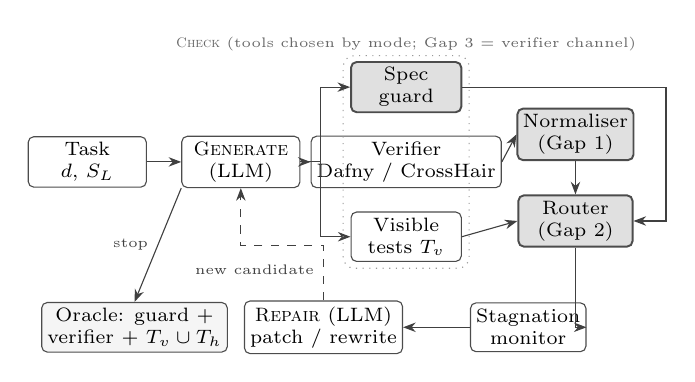
\begin{tikzpicture}[
  font=\scriptsize,
  box/.style={draw=black!70, rounded corners=2pt, align=center, minimum height=0.62cm, inner sep=2pt, fill=white},
  gap/.style={box, fill=black!12, line width=0.7pt},
  arr/.style={-{Stealth[length=1.6mm]}, black!75},
  fb/.style={-{Stealth[length=1.6mm]}, black!75, dashed}
]
\node[box, minimum width=1.5cm] (task) at (0,0) {Task\\ $d$, $S_L$};
\node[box, minimum width=1.5cm] (gen) at (1.95,0) {\textsc{Generate}\\ (LLM)};
\node[gap, minimum width=1.4cm] (guard) at (4.05,0.95) {Spec\\ guard};
\node[box, minimum width=1.4cm] (ver) at (4.05,0) {Verifier\\ Dafny / CrossHair};
\node[box, minimum width=1.4cm] (tst) at (4.05,-0.95) {Visible\\ tests $T_v$};
\node[gap, minimum width=1.45cm] (norm) at (6.2,0.35) {Normaliser\\ (Gap 1)};
\node[gap, minimum width=1.45cm] (route) at (6.2,-0.75) {Router\\ (Gap 2)};
\node[box, minimum width=1.5cm] (rep) at (3.0,-2.1) {\textsc{Repair} (LLM)\\ patch / rewrite};
\node[box, minimum width=1.4cm] (stag) at (5.6,-2.1) {Stagnation\\ monitor};
\node[box, minimum width=1.5cm, fill=black!4] (orc) at (0.6,-2.1) {Oracle: guard +\\ verifier + $T_v\cup T_h$};

\draw[arr] (task) -- (gen);
\draw[arr] (gen.east) -- ++(0.25,0) |- (guard.west);
\draw[arr] (gen.east) -- (ver.west);
\draw[arr] (gen.east) -- ++(0.25,0) |- (tst.west);
\draw[arr] (ver.east) -- (norm.west);
\draw[arr] (norm.south) -- (route.north);
\draw[arr] (tst.east) -- (route.west);
\draw[arr] (guard.east) -| ([xshift=4mm]norm.east) |- (route.east);
\draw[arr] (route.south) |- (stag.east);
\draw[arr] (stag.west) -- (rep.east);
\draw[fb] (rep.north) -- node[left, pos=0.55, font=\tiny] {new candidate} ++(0,0.7) -| (gen.south);
\draw[arr] (gen.south west) -- node[left, font=\tiny, align=right] {stop} (orc.north);
\node[font=\tiny, black!60] at (4.05,1.5) {\textsc{Check} (tools chosen by mode; Gap 3 = verifier channel)};
\draw[black!40, dotted, rounded corners] (3.25,-1.35) rectangle (4.85,1.35);
\end{tikzpicture}
}
\caption{SpecLoop architecture. Shaded boxes are the gap-specific components, each of which can be switched off. The oracle is outside the agent and judges every candidate in the same way.}
\label{fig:arch}
\end{figure}

\subsection{Tools and environment}
The agent works against two real toolchains. For Dafny it calls \texttt{dafny verify} (Dafny 4.11 with its bundled Z3~\cite{demoura2008z3}, 20\,s per verification condition) and, for tests, compiles the program together with a generated \texttt{Main} method to Python and runs it. For Python it runs CrossHair~\cite{crosshair} in iContract mode (6\,s per condition) and executes the tests with contracts enabled, so a violated postcondition shows up as a failing test. Test cases are stored once in a language-neutral JSON form and rendered into both languages, so the two versions of a task see exactly the same inputs and expected outputs. Tool results are memoised by program hash, so resubmitting an identical program does not cost another verifier run.

\subsection{Gap 1 component: diagnostic normaliser}
Dafny and CrossHair report problems in very different shapes. Dafny gives a file position, a message such as ``a postcondition could not be proved on this return path'' and a separate ``related location'' that points at the clause. CrossHair reports the line of the violated contract and a concrete call. Neither output is easy for a model to use directly, because both refer to line numbers in a file the model never sees. The normaliser maps both into one taxonomy (\texttt{syntax}, \texttt{resolution}, \texttt{postcondition}, \texttt{invariant\_entry}, \texttt{invariant\_maintained}, \texttt{termination}, \texttt{index\_bounds}, \texttt{counterexample}, \texttt{exception}, \texttt{timeout}), quotes the offending source line and the specification clause involved, and adds a one-line explanation of each kind. With this in place, one agent loop runs unchanged on both languages. With the component off, the model receives the raw tool output with temporary paths removed, which is what the Phase~1 prototype did.

\subsection{Gap 2 component: feedback router}
The router starts from one observation. A Dafny error such as ``postcondition could not be proved'' is ambiguous, since Dafny reports it both when the program is wrong and when the program is right but the loop invariants are missing. Tests can separate the two cases cheaply. The router therefore classifies every failed check:
\textsc{spec\_tamper} (the guard fired), \textsc{syntax} (does not compile), \textsc{logic\_bug} (a visible test fails or CrossHair produced a counterexample), and \textsc{proof\_gap} (all visible tests pass but verification fails). Each class comes with a different instruction. For a logic bug the model is told to fix the algorithm first and is shown failing tests before verifier messages. For a proof gap it is told to keep the algorithm and strengthen loop invariants, \texttt{decreases} clauses or assertions. For a compile error the model sees only the compile errors. With the router off, SpecLoop pastes the verifier output and the test output one after the other, as the Phase~1 combined agent did.

\subsection{Gap 3 component: verifier feedback channel}
Gap~3 is about the verifier signal itself, so its component is just the verifier channel in \textsc{Check}. Removing it turns SpecLoop into the testing-only agent, which is our E1 baseline and the configuration VERINA does not have.

\subsection{Specification integrity guard}
\label{sec:guard}
A program that edits its own specification can be ``verified'' and still be wrong. The guard compares each candidate with the original specification before any tool runs. For Dafny it strips comments, normalises whitespace and requires the target method header (signature and every \texttt{requires}/\texttt{ensures} clause) and every other declaration from the specification file to appear unchanged. It also rejects \texttt{assume}, \texttt{\{:axiom\}}, \texttt{\{:verify false\}}, \texttt{\{:only\}}, \texttt{\{:extern\}} and \texttt{decreases *}, and any Dafny warning about bodyless lemmas. For Python it compares abstract syntax trees, so formatting does not matter, and requires identical decorators, signature, imports and helper definitions. CrossHair directive comments, assignments to the \texttt{icontract} module, \texttt{eval}/\texttt{exec} and access to \texttt{sys.modules} are rejected as well. A rejected candidate is not verified at all. The model is told exactly what it changed and has to restore it. Even when the in-loop guard is switched off, the oracle applies the same guard to every final program, so no configuration can gain correctness by cheating.

\subsection{Stagnation monitor}
In early development runs the loop often got stuck. The model resubmitted an identical program, or produced new programs that failed in exactly the same way. The monitor fingerprints each failure (class, diagnostic kinds and lines, failing test indices) and, when an identical program is resubmitted or the same fingerprint appears twice in a row, switches the next call to a \emph{rewrite}: the prompt asks for a fresh approach and the temperature is raised from 0.2 to 0.6.

\subsection{Observability}
Each run writes a trajectory with state transitions, every LLM call (tokens, the model's analysis and strategy, the program), every tool call (input hash, status, diagnostics, time), the routed feedback and its class, and each stop or strategy decision. The oracle also gives a verdict for every candidate, and these per-candidate verdicts let us compute correctness after $k$ attempts for every $k \le K$ from a single run.

\section{Experimental Setup}
\label{sec:setup}

\textbf{Benchmark.} We rebuilt the Phase~1 benchmark from the base paper's own data. VERINA-BASIC has 108 tasks, all of which the VERINA authors translated into Lean from Dafny originals in CloverBench (59) and MBPP-DFY (49). We kept every task whose types have a direct counterpart in both Dafny and Python (integers, naturals, booleans, characters, strings, lists and tuples), which left 97 tasks after removing ten with floats, options, maps, bytes, function arguments or nested arrays, and one malformed record. For each remaining task we wrote a Dafny specification, a Python/iContract specification and a reference solution in each language, using VERINA's Lean pre- and postcondition as the ground truth for what the task means and VERINA's positive tests as our tests (2 to 12 per task, median 5). A task was admitted only if, in both languages, (i) the reference passes the integrity guard, (ii) it verifies, (iii) it passes all tests, (iv) the empty stub is rejected, and (v) the specification accepts the expected output and rejects every known-wrong output that VERINA lists for each test input. We call check (v) a \emph{spec probe}. In Dafny, a probe is a copy of the method with the test input pinned by extra \texttt{requires} clauses and a body that returns the candidate output. Because both specifications answer the same concrete questions, the probes are our main evidence that the two versions of a task are equivalent. As a second check we ran both references on random inputs that satisfy the precondition and compared their outputs (differential testing). All 97 tasks passed the five checks in both languages; for three Dafny tasks the verifier could not decide some accept-probes on literal inputs, and these exemptions are documented in the task files. Differential testing on \R{eq.inputs} random inputs found no disagreement between the Dafny and Python references.

\textbf{Splits.} Before any experiment we drew 20 tasks at random (seed 2026) as a development split and kept the remaining 77 as the test split. All design decisions (five development iterations, recorded in the repository's development log), the prompts, and the two worked examples used by E2 come from the development split only. Every number in Sections~\ref{sec:results}--\ref{sec:failures} is on the test split, which gives 154 task instances (77 per language).

\textbf{Model and decoding.} All experiments use \texttt{gpt-4o-mini-2024-07-18}, one of the models VERINA evaluates, which makes the base-paper comparison like for like. We had planned to add GPT-4.1, but the project had a hard budget of 2~USD for API calls, so the stronger model could not be run at the scale we needed (Section~\ref{sec:limits}). Agents use temperature 0.2 (0.6 for rewrites), at most 4096 output tokens, OpenAI seeds 0, 1 and 2 for the three repetitions, and a budget of $K = 5$ candidates. Every request and response is stored in a cache keyed on the full request, so all runs can be replayed exactly without new API calls.

\textbf{Experiments.} E1 runs the Phase~1 baselines (single-shot and testing-only). E2 reproduces VERINA's CodeGen protocol on our tasks, with the same instruction structure (task description plus a template that contains the reference specification), two worked examples, temperature 1.0 and plain-text answers. Because of the budget we drew 3 samples per task instead of VERINA's 5, but pass@1 is still estimated without bias as the mean over samples~\cite{chen2021codex}. E3 runs the full SpecLoop agent, and E4 adds the verifier-only arm and reuses E1 and E3 for the gap-wise tests. In E5 we remove one component at a time from SpecLoop. Finally, E6 collects cost, latency, tool usage and reliability measures from all runs, together with a stress test of the integrity guard.

\textbf{Implementation.} SpecLoop is about 4,200 lines of Python. Experiments ran on a 16-core Windows~10 machine with Dafny~4.11.0, CrossHair~0.0.113 and Python~3.12, with up to 6 runs in parallel per experiment. The code, task files, raw results, trajectories and the scripts that produce every table and figure are in the project repository.

\section{Evaluation Methodology}
\label{sec:eval}

\textbf{Metrics.} Our primary metric is \emph{correctness}, the share of runs whose final program satisfies Eq.~(1). We also report the \emph{verified rate} (the verifier accepts the final program), the \emph{test pass rate} on all tests, VERINA's CodeGen metric (pass@1 on tests, with the share of samples that do not compile), and the \emph{spec-intact rate}. For reliability we report the \emph{false-success rate}, the share of runs where the agent stopped because its own checks passed but the oracle disagrees (possible when a testing-only agent never sees the verifier, or when the in-loop guard is off). For efficiency we count model calls, tokens, cost in USD, verifier and test calls, and wall-clock time per run. Per-candidate oracle verdicts give \emph{correct@$k$}, the correctness an agent would reach with a budget of $k$ candidates.

\textbf{Statistics.} Each configuration is run three times, and we report the mean and standard deviation over the three runs. For comparisons between configurations we pair results by task: we average each task's outcome over seeds and apply a Wilcoxon signed-rank test~\cite{wilcoxon1945individual} to the per-task differences, and as a second check an exact McNemar test~\cite{mcnemar1947note} on matched (task, seed) outcomes. We also give 95\% bootstrap confidence intervals for the difference in rates. For Gap~1 the pairing is by VERINA task across the two languages. We use $\alpha = 0.05$ and do not correct for multiple comparisons, so p-values near the threshold should be read with care.

\textbf{Base-paper comparison.} We compare against VERINA in two ways and keep them apart in every table. \emph{Reported} numbers are VERINA's own GPT-4o-mini results on VERINA-BASIC in Lean (Table~9 of~\cite{ye2026verina}: 44.0\% pass@1, 54.9\% of samples do not compile). \emph{Reproduced} numbers come from E2, which runs VERINA's protocol with the same model on our Dafny and Python versions of the same tasks. The difference between the two isolates the effect of the specification language, and the difference between E2 and our agents isolates the effect of the feedback loop.

\section{Results}
\label{sec:results}

Table~\ref{tab:main} gives the main results on the 77 test tasks in each language. Every configuration starts from the same first candidate for a given task and seed, so the single-shot row is also the starting point of every loop.

\begin{table}[t]
\centering
\caption{Main results on the test split (GPT-4o-mini, 77 tasks per language, 3 seeds). Correct = spec intact, verified and all tests pass (mean $\pm$ s.d.\ over seeds, \%). Ver = verified, Tests = passes all tests (visible and held-out).}
\label{tab:main}
\footnotesize
\setlength{\tabcolsep}{3.2pt}
\begin{tabular}{lccc|ccc}
\toprule
 & \multicolumn{3}{c|}{Dafny} & \multicolumn{3}{c}{Python/iContract} \\
Configuration & Correct & Ver & Tests & Correct & Ver & Tests \\
\midrule
Single-shot (E1) & \R{dafny.single_shot.correct}$\pm$\R{dafny.single_shot.correctsd} & \R{dafny.single_shot.verified} & \R{dafny.single_shot.tests} & \R{python.single_shot.correct}$\pm$\R{python.single_shot.correctsd} & \R{python.single_shot.verified} & \R{python.single_shot.tests} \\
Testing-only (E1) & \R{dafny.testing_only.correct}$\pm$\R{dafny.testing_only.correctsd} & \R{dafny.testing_only.verified} & \R{dafny.testing_only.tests} & \R{python.testing_only.correct}$\pm$\R{python.testing_only.correctsd} & \R{python.testing_only.verified} & \R{python.testing_only.tests} \\
Verifier-only (E4) & \R{dafny.verifier_only.correct}$\pm$\R{dafny.verifier_only.correctsd} & \R{dafny.verifier_only.verified} & \R{dafny.verifier_only.tests} & \R{python.verifier_only.correct}$\pm$\R{python.verifier_only.correctsd} & \R{python.verifier_only.verified} & \R{python.verifier_only.tests} \\
SpecLoop (E3) & \textbf{\R{dafny.specloop_full.correct}}$\pm$\R{dafny.specloop_full.correctsd} & \R{dafny.specloop_full.verified} & \R{dafny.specloop_full.tests} & \R{python.specloop_full.correct}$\pm$\R{python.specloop_full.correctsd} & \R{python.specloop_full.verified} & \R{python.specloop_full.tests} \\
\bottomrule
\end{tabular}
\end{table}


\subsection{Comparison with the base paper (E1, E2)}
Table~\ref{tab:e2} puts VERINA's reported numbers next to our reproduction of its protocol. With the same model and the same tasks, moving from Lean to Dafny raises the share of samples that pass all tests from \R{etwo.verina.pass}\% to \R{etwo.dafny.pass}\%, and moving to Python raises it to \R{etwo.python.pass}\%. Most of the difference is compilation: \R{etwo.verina.nocompile}\% of VERINA's GPT-4o-mini programs do not compile in Lean, against \R{etwo.dafny.nocompile}\% in Dafny and \R{etwo.python.nocompile}\% in Python. VERINA's CodeGen metric does not ask for a proof, though. Once we also require the program to verify, Dafny falls to \R{etwo.dafny.correct}\%, which is close to the Lean pass rate, while Python stays at \R{etwo.python.correct}\%. Our own single-shot prompt (temperature 0.2, no worked examples) gives \R{dafny.single_shot.correct}\% on Dafny, in the same range as the 2-shot protocol.

\begin{table}[t]
\centering
\caption{Base paper vs.\ reproduction (GPT-4o-mini, single attempt). VERINA numbers are \emph{reported} (Lean, Table~9 of~\cite{ye2026verina}); Dafny and Python are \emph{reproduced} with VERINA's protocol on our versions of the same tasks (E2, 3 samples per task).}
\label{tab:e2}
\footnotesize
\begin{tabular}{lcccc}
\toprule
Setting & Pass@1 & No compile & Verified@1 & Correct@1 \\
\midrule
VERINA, Lean (reported) & \R{etwo.verina.pass} & \R{etwo.verina.nocompile} & n/a & n/a \\
E2, Dafny (reproduced) & \R{etwo.dafny.pass} & \R{etwo.dafny.nocompile} & \R{etwo.dafny.verified} & \R{etwo.dafny.correct} \\
E2, Python (reproduced) & \R{etwo.python.pass} & \R{etwo.python.nocompile} & \R{etwo.python.verified} & \R{etwo.python.correct} \\
\bottomrule
\end{tabular}
\end{table}

\subsection{RQ1: specification language (Gap 1)}
The language effect is larger than any feedback effect we measured. Paired by task, Python/iContract is ahead of Dafny in every configuration, from \R{gap1.single_shot.correct.diff}~pp for single-shot generation (95\% CI [\R{gap1.single_shot.correct.lo}, \R{gap1.single_shot.correct.hi}], Wilcoxon \emph{p}~\R{gap1.single_shot.correct.p}) to \R{gap1.specloop_full.correct.diff}~pp for SpecLoop (\emph{p}~\R{gap1.specloop_full.correct.p}). Out of 231 matched task-seed pairs under SpecLoop, Dafny is correct where Python is not in only \R{gap1.specloop_full.correct.aonly} cases, and the reverse happens \R{gap1.specloop_full.correct.bonly} times.

H1a predicted the opposite of what we found: Dafny's verification rate is lower, not higher (\R{dafny.specloop_full.verified}\% against \R{python.specloop_full.verified}\% under SpecLoop). H1b holds: the first candidate passes all tests for \R{dafny.single_shot.tests}\% of Dafny instances and \R{python.single_shot.tests}\% of Python instances (\emph{p}~\R{gap1.first_attempt_tests_ok.p}). Two things drive the gap. Dafny programs fail to compile far more often (Table~\ref{tab:e2}), and even a Dafny program that computes the right answers still needs loop invariants strong enough for the verifier. Under testing-only feedback \R{dafny.testing_only.tests}\% of Dafny programs pass every test but only \R{dafny.testing_only.verified}\% verify. In Python the two rates are almost the same, partly because CrossHair gives a weaker, bounded guarantee (Section~\ref{sec:limits}). For a team that only needs contracts checked to this standard, Python with iContract is the far easier target. For a team that needs a proof, Dafny delivers one for roughly two thirds of these small tasks after feedback, which is still well above what VERINA reports for proofs in Lean.

\subsection{RQ2: combining verifier and test feedback (Gap 2)}
On Dafny, SpecLoop is the best configuration. It is \R{gap2.dafny.full_vs_verifier.diff}~pp above the verifier-only agent (95\% CI [\R{gap2.dafny.full_vs_verifier.lo}, \R{gap2.dafny.full_vs_verifier.hi}]; McNemar \emph{p}~\R{gap2.dafny.full_vs_verifier.pm}, Wilcoxon \emph{p}~\R{gap2.dafny.full_vs_verifier.p}) and \R{gap2.dafny.full_vs_testing.diff}~pp above the testing-only agent (\emph{p}~\R{gap2.dafny.full_vs_testing.p}). Against the verifier-only agent it wins on \R{gap2.dafny.full_vs_verifier.aonly} task-seed pairs and loses on \R{gap2.dafny.full_vs_verifier.bonly}. The gain over the better single-source agent is just under the 5~pp we set in H2, and the two tests disagree on significance at $\alpha = 0.05$. We therefore count H2 as partly supported. On Python all three loops sit at the ceiling and the differences are zero or within one task.

The verifier-only runs show why tests help. Of the \R{ambig.dafny.fails} failed Dafny verifications in those runs, \R{ambig.dafny.prooffails} (\R{ambig.dafny.share}\%) were on programs that already passed every test, visible and held-out. For these programs the verifier's message (usually ``a postcondition could not be proved'') was correct but misleading: the code was right and only the proof was missing, yet the agent had no way to know that. SpecLoop's router uses the visible tests to label such cases \textsc{proof\_gap} and asks for stronger invariants instead of a new algorithm. This is also why the combined loop needs fewer model calls than the verifier-only loop (\R{dafny.specloop_full.calls} vs.\ \R{dafny.verifier_only.calls} per run).

\subsection{RQ3: what the verifier adds over tests (Gap 3)}
The testing-only agent is the baseline VERINA does not have. On Dafny it improves on single-shot generation (\R{dafny.testing_only.correct}\% against \R{dafny.single_shot.correct}\%), which shows that test feedback alone is useful. Adding the verifier channel raises correctness by a further \R{gap3.dafny.verifier_vs_testing.diff}~pp (verifier-only against testing-only, 95\% CI [\R{gap3.dafny.verifier_vs_testing.lo}, \R{gap3.dafny.verifier_vs_testing.hi}], \emph{p}~\R{gap3.dafny.verifier_vs_testing.p}), and by \R{gap3.dafny.full_vs_testing.diff}~pp when tests are kept as well (SpecLoop against testing-only). The gain is significant but smaller than the 10~pp we predicted in H3, so H3 is partly supported.

The more important difference is in what the agents believe when they stop. The testing-only agent stops as soon as its visible tests pass, and in \R{dafny.testing_only.falsesuccess}\% of its Dafny runs (\R{rel.testing_only.falsesuccess} runs over both languages) it stopped with a program that the oracle rejects. In every one of these runs the program passed all tests, including the held-out ones, but did not verify, so the agent had no signal that anything was missing. No run of an agent with verifier feedback ended this way. In other words, a test-driven agent cannot tell the user how reliable its answer is, while an agent that sees the verifier can. With only one model in our budget (Section~\ref{sec:limits}), we could not test whether this gain changes with model strength.

\subsection{Gap-resolution summary}
Table~\ref{tab:gapres} summarises the three gaps.

\begin{table*}[t]
\centering
\caption{Gap-resolution table (Dafny unless noted; Python is at ceiling for every configuration). $\Delta$ in percentage points with 95\% bootstrap CI and Wilcoxon $p$ over tasks.}
\label{tab:gapres}
\footnotesize
\begin{tabular}{p{0.06\textwidth}p{0.2\textwidth}p{0.15\textwidth}p{0.17\textwidth}p{0.22\textwidth}p{0.11\textwidth}}
\toprule
Gap & Method / component & Metric & Base paper result & Our result & Addressed? \\
\midrule
Gap 1 & Same tasks in Dafny and Python/iContract (probe-checked specs); multi-backend verification with the diagnostic normaliser & CodeGen pass@1; correctness & Lean: \R{etwo.verina.pass}\% pass@1, \R{etwo.verina.nocompile}\% do not compile (reported) & Pass@1 Dafny \R{etwo.dafny.pass}\%, Python \R{etwo.python.pass}\%; SpecLoop correct Dafny \R{dafny.specloop_full.correct}\%, Python \R{python.specloop_full.correct}\% ($\Delta$ \R{gap1.specloop_full.correct.diff}, \emph{p}~\R{gap1.specloop_full.correct.p}) & Fully (H1a refuted, H1b supported) \\
Gap 2 & Test channel + feedback router (\textsc{logic\_bug} vs.\ \textsc{proof\_gap}) & Correctness vs.\ best single source & Not studied (single-shot only) & SpecLoop \R{dafny.specloop_full.correct}\% vs.\ verifier-only \R{dafny.verifier_only.correct}\% ($\Delta$ \R{gap2.dafny.full_vs_verifier.diff} [\R{gap2.dafny.full_vs_verifier.lo}, \R{gap2.dafny.full_vs_verifier.hi}], McNemar \emph{p}~\R{gap2.dafny.full_vs_verifier.pm}) & Partially (gain below 5~pp target) \\
Gap 3 & Verifier feedback channel vs.\ identical testing-only agent & Correctness gain; false-success rate & No testing-only baseline & $\Delta$ \R{gap3.dafny.verifier_vs_testing.diff} [\R{gap3.dafny.verifier_vs_testing.lo}, \R{gap3.dafny.verifier_vs_testing.hi}], \emph{p}~\R{gap3.dafny.verifier_vs_testing.p}; false success \R{dafny.testing_only.falsesuccess}\% vs.\ 0\% & Partially (gain below 10~pp target; one model) \\
\bottomrule
\end{tabular}
\end{table*}

\section{Ablation and Comparative Analysis}
\label{sec:ablation}

\textbf{Ablation (E5).} Table~\ref{tab:ablation} removes one component at a time from SpecLoop on Dafny. Python is left out because the shared first candidate already solves about 96\% of the Python instances, so no component can change the outcome there. When SpecLoop's first candidate passes every check, every combined-mode variant stops at that same candidate with the same verdict. We therefore executed each variant only on the units where SpecLoop needed feedback (\R{e5.executed} of the \R{e5.total} Dafny units per variant) and reused the identical first-attempt result for the rest. Removing the test channel gives the verifier-only agent and removing the verifier channel gives the testing-only agent, so those two rows come from E4 and E1.

\begin{table}[t]
\centering
\caption{Ablation on Dafny (E5): correctness when one component is removed (mean $\pm$ s.d.\ over 3 seeds, \%). $\Delta$ is the paired difference to the full system in percentage points with 95\% bootstrap CI.}
\label{tab:ablation}
\footnotesize
\setlength{\tabcolsep}{3pt}
\begin{tabular}{lccc}
\toprule
Variant & Correct & $\Delta$ [95\% CI] & $p$ \\
\midrule
Full SpecLoop & \R{abl.dafny.fullsystem.correct}$\pm$\R{abl.dafny.fullsystem.sd} & -- & -- \\
-- normaliser (raw output) & \R{abl.dafny.no_normalizer.correct}$\pm$\R{abl.dafny.no_normalizer.sd} & \R{abl.dafny.no_normalizer.delta} [\R{abl.dafny.no_normalizer.lo}, \R{abl.dafny.no_normalizer.hi}] & \R{abl.dafny.no_normalizer.p} \\
-- router (plain concatenation) & \R{abl.dafny.no_router.correct}$\pm$\R{abl.dafny.no_router.sd} & \R{abl.dafny.no_router.delta} [\R{abl.dafny.no_router.lo}, \R{abl.dafny.no_router.hi}] & \R{abl.dafny.no_router.p} \\
-- guard in the loop & \R{abl.dafny.no_guard.correct}$\pm$\R{abl.dafny.no_guard.sd} & \R{abl.dafny.no_guard.delta} [\R{abl.dafny.no_guard.lo}, \R{abl.dafny.no_guard.hi}] & \R{abl.dafny.no_guard.p} \\
-- stagnation monitor & \R{abl.dafny.no_stagnation.correct}$\pm$\R{abl.dafny.no_stagnation.sd} & \R{abl.dafny.no_stagnation.delta} [\R{abl.dafny.no_stagnation.lo}, \R{abl.dafny.no_stagnation.hi}] & \R{abl.dafny.no_stagnation.p} \\
-- dev fixes (iterations 4--5) & \R{abl.dafny.no_dev_fixes.correct}$\pm$\R{abl.dafny.no_dev_fixes.sd} & \R{abl.dafny.no_dev_fixes.delta} [\R{abl.dafny.no_dev_fixes.lo}, \R{abl.dafny.no_dev_fixes.hi}] & \R{abl.dafny.no_dev_fixes.p} \\
-- test channel (= verifier-only) & \R{abl.dafny.no_test_channel.correct}$\pm$\R{abl.dafny.no_test_channel.sd} & \R{abl.dafny.no_test_channel.delta} [\R{abl.dafny.no_test_channel.lo}, \R{abl.dafny.no_test_channel.hi}] & \R{abl.dafny.no_test_channel.p} \\
-- verifier channel (= testing-only) & \R{abl.dafny.no_verifier_channel.correct}$\pm$\R{abl.dafny.no_verifier_channel.sd} & \R{abl.dafny.no_verifier_channel.delta} [\R{abl.dafny.no_verifier_channel.lo}, \R{abl.dafny.no_verifier_channel.hi}] & \R{abl.dafny.no_verifier_channel.p} \\
\bottomrule
\end{tabular}
\end{table}

The verifier channel is the most important single part: without it correctness falls by \R{abl.dafny.no_verifier_channel.delta}~pp (\emph{p}~\R{abl.dafny.no_verifier_channel.p}). The diagnostic normaliser comes next. Replacing its structured messages with raw Dafny output costs \R{abl.dafny.no_normalizer.delta}~pp (\emph{p}~\R{abl.dafny.no_normalizer.p}), and removing the fix hints and loop checks added in development iterations 4 and 5 costs \R{abl.dafny.no_dev_fixes.delta}~pp (\emph{p}~\R{abl.dafny.no_dev_fixes.p}). Neither effect was visible on the 20 development tasks with one seed (Section~\ref{sec:limits}), so the test split confirms decisions that the dev split could only suggest. Removing the test channel costs \R{abl.dafny.no_test_channel.delta}~pp and removing the router \R{abl.dafny.no_router.delta}~pp; both point in the expected direction, but neither is significant on its own, which matches the modest RQ2 effect. The stagnation monitor adds about one point (\R{abl.dafny.no_stagnation.delta}~pp, \emph{p}~\R{abl.dafny.no_stagnation.p}). Switching the in-loop guard off changes nothing at all, because GPT-4o-mini almost never edited the specification in these runs; the guard matters for validity, not for accuracy (see below).

\textbf{Attempt budget.} Fig.~\ref{fig:curves} shows correctness as a function of the number of candidates $k$. On Dafny all three loops start from the same point (\R{curve.dafny.specloop_full.k1}\% at $k=1$) and separate after the first round of feedback. The testing-only curve is almost flat after $k=2$ (\R{curve.dafny.testing_only.k2}\% to \R{curve.dafny.testing_only.k5}\%), since once the visible tests pass it has nothing left to fix. The verifier-only curve rises to \R{curve.dafny.verifier_only.k5}\%, and SpecLoop rises fastest and is still gaining at $k=5$ (\R{curve.dafny.specloop_full.k4}\% to \R{curve.dafny.specloop_full.k5}\%), so a larger budget would probably help it more than the others. Across three seeds SpecLoop turned \R{repaired.dafny.specloop_full} failing first candidates into correct Dafny programs, against \R{repaired.dafny.verifier_only} for verifier-only and \R{repaired.dafny.testing_only} for testing-only.

\begin{figure}[t]
\centering
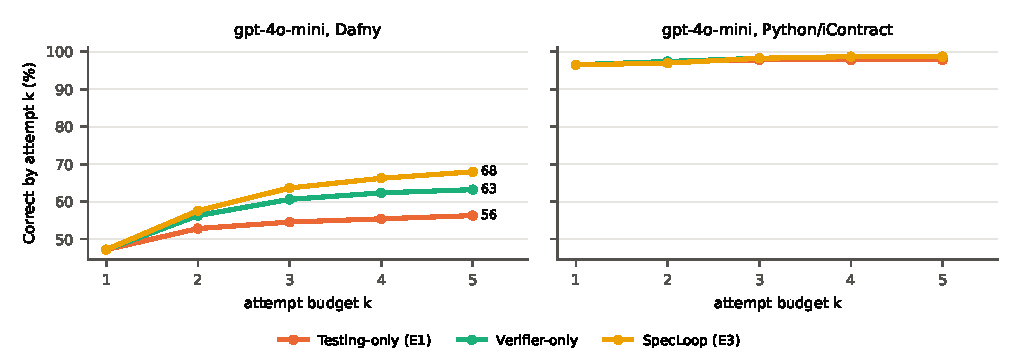
\includegraphics[width=\columnwidth]{generated/fig_curves.pdf}
\caption{Correctness after $k$ candidates (from per-candidate oracle verdicts). All configurations share the first candidate, so they start from the same point at $k=1$.}
\label{fig:curves}
\end{figure}

\textbf{Efficiency (E6).} On Dafny a run costs \R{dafny.single_shot.costrun}~m\$ (thousandths of a dollar) for single-shot generation, \R{dafny.testing_only.costrun}~m\$ for testing-only, \R{dafny.verifier_only.costrun}~m\$ for verifier-only and \R{dafny.specloop_full.costrun}~m\$ for SpecLoop, with \R{dafny.single_shot.calls}, \R{dafny.testing_only.calls}, \R{dafny.verifier_only.calls} and \R{dafny.specloop_full.calls} model calls per run on average. The cost that matters, though, is the cost per correct program. There, SpecLoop (\R{dafny.specloop_full.costsolved}~m\$) is cheaper than the verifier-only agent (\R{dafny.verifier_only.costsolved}~m\$), because the router lets it solve more tasks with slightly fewer calls. The testing-only agent is cheaper still per solved task (\R{dafny.testing_only.costsolved}~m\$), but it reaches a lower ceiling and, as shown above, cannot tell when its answer is unverified. Verification dominates the latency of the verifier-based loops: tool time is \R{rel.specloop_full.toolshare}\% of SpecLoop's model-plus-tool time, against \R{rel.testing_only.toolshare}\% for testing-only. On Python every configuration costs about the same, since nearly all runs end after one candidate. The whole study, including development runs and E2, cost \R{total.allspend}~USD in API calls.


\textbf{Reliability and the integrity guard (E6).} To test whether ``verified'' can be trusted, we built tampered versions of every reference solution: a dropped or weakened \texttt{ensures}, an added \texttt{requires false}, \texttt{assume false}, \texttt{\{:verify false\}}, an axiom lemma, an edited helper predicate, a removed or weakened iContract decorator, an added \texttt{require(lambda \ldots: False)}, a CrossHair-off comment, and a patched \texttt{icontract}. We also built harmless variants that only reformat or add comments. The guard rejected all \R{guard.dafny.tamper.n} Dafny and all \R{guard.python.tamper.n} Python tampering mutants and none of the \R{guard.dafny.benign.n} plus \R{guard.python.benign.n} harmless ones. Without the guard the result would have looked very different: Dafny alone accepted \R{guard.dafny.tamper.veraccepts} of the \R{guard.dafny.tamper.n} tampered programs, and CrossHair accepted \R{guard.python.tamper.veraccepts} of the \R{guard.python.tamper.checked} Python mutants we ran through it. In the actual runs GPT-4o-mini rarely tried to change the specification (the in-loop guard fired in \R{rel.specloop_full.runswithguardblock} SpecLoop run), so the guard is mostly insurance, but it is what lets us report a verified program as correct. The stagnation monitor switched to a rewrite in \R{rel.specloop_full.runswithswitch} SpecLoop runs, and \R{rel.specloop_full.solvedafterswitch} of those ended correct.

\section{Failure Analysis}
\label{sec:failures}

We took every run of the full system that ended without a correct program and assigned it to one category, using the last oracle verdict, the last verifier diagnostics and the final program. The categories and their frequencies are shown in Fig.~\ref{fig:failures}.

\begin{figure}[t]
\centering
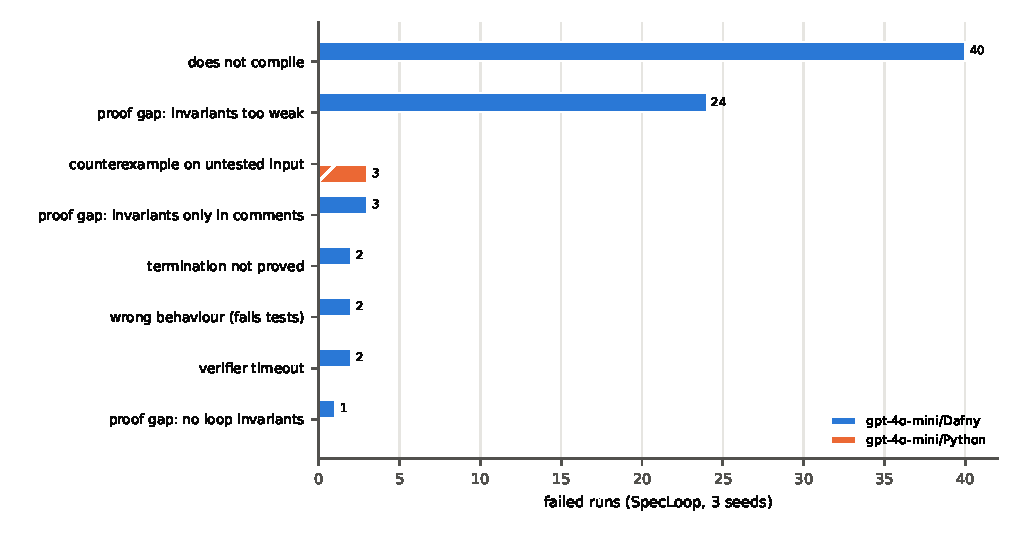
\includegraphics[width=\columnwidth]{generated/fig_failures.pdf}
\caption{Failure categories of the full SpecLoop agent on the test split (all failed runs over three seeds).}
\label{fig:failures}
\end{figure}

Over three seeds the full agent failed \R{fail.dafny.total} Dafny runs and \R{fail.python.total} Python runs. Four categories cover almost all of them.

\textbf{Does not compile (\R{fail.dafny.DoesNotCompile} Dafny runs, \R{fail.dafny.DoesNotCompile.share}\%).} The most frequent failure is a program that never compiles, even after four repairs. The errors are the ones that motivated development iteration~4: array operations on sequences, string building with constructs Dafny does not have, statement \texttt{if} written with \texttt{then}, and calls to library functions that do not exist. The fix hints help (vb\_017, vb\_082 and vb\_105 were solved on the dev split only after they were added), but GPT-4o-mini often swaps one compile error for another instead of converging. This mirrors VERINA, where most GPT-4o-mini failures were Lean compile errors. Better language grounding, for example retrieving short Dafny idioms for the construct that failed, is the obvious next step.

\textbf{Proof gap (\R{fail.dafny.ProofGapInvariantsTooWeak} + \R{fail.dafny.ProofGapInvariantsOnlyInComments} + \R{fail.dafny.ProofGapNoLoopInvariants} runs).} The program passes every test but does not verify. In most of these runs the invariants exist but are too weak to imply the postcondition, typically a bound on the index without a clause that relates the partial result to the specification. A few runs still write the invariants as comments or leave them out entirely. Here the router does its job and labels these attempts \textsc{proof\_gap}, but the model does not know how to strengthen the invariant. Invariant-generation techniques such as those in Lemur~\cite{wu2024lemur} or Laurel~\cite{mugnier2025laurel} would slot into exactly this branch of the loop.

\textbf{Termination and timeouts (\R{fail.dafny.TerminationNotProved} + \R{fail.dafny.VerifierTimeout} runs).} Missing \texttt{decreases} clauses and quantifier-heavy invariants that exhaust the verifier's time limit are rare with these small tasks.

\textbf{Wrong behaviour and counterexamples (\R{fail.dafny.WrongBehaviourFailsTests} Dafny, \R{fail.python.CounterexampleOnUntestedInput} Python runs).} Very few runs end with code that is actually wrong. In Python every failure is a program that passes all tests but for which CrossHair finds an input that breaks a contract, which is precisely the kind of error the verifier is there to catch.

\textbf{Representative cases.} The trajectories are in \texttt{results/cases/} of the repository. \emph{Success 1} (vb\_016, Dafny, replace characters): the first candidate does not compile (array syntax on a sequence) and is routed as \textsc{syntax}. The second compiles and passes every visible test but does not verify, so the router labels it \textsc{proof\_gap}. The model keeps the algorithm, adds an invariant that ties the partial result to the input, and the third candidate verifies. \emph{Success 2} (vb\_033, Python, smallest missing number): the first candidate passes all five tests, but CrossHair finds a sorted input with duplicates that breaks the postcondition (\textsc{logic\_bug}). The next candidate fails in the same way, the stagnation monitor switches to a rewrite, and the rewritten set-based version is correct. A testing-only agent would have stopped at the first, wrong program. \emph{Failure 1} (vb\_009, Dafny, common element): the code is right from the first attempt and passes all eight tests, but all five candidates fail on invariants about the multiset of seen elements; each repair changes the invariants without making them strong enough. \emph{Failure 2} (vb\_086, Dafny, rotate a sequence): the first candidate tries to fill an array where the specification works with sequences, the second and third use a comprehension syntax that does not exist in Dafny, and the fourth goes back to a resolution error. All four are routed as \textsc{syntax}. The fifth candidate finally compiles but rotates in the wrong direction and passes only one of six tests.

\section{Limitations and Threats to Validity}
\label{sec:limits}

\textbf{One model.} The API budget for the whole project was 2~USD, so every experiment uses GPT-4o-mini. This keeps the base-paper comparison exact, since VERINA reports the same checkpoint, but it leaves RQ3's secondary question (does the gain hold across models) open. A stronger model might make fewer compile errors and more proof gaps, which would shift the weight between components. The agent works with any OpenAI-compatible endpoint, and the cache makes adding a model cheap.

\textbf{Unequal verifiers.} Dafny proves the postcondition for all inputs, while CrossHair only searches for a counterexample for a fixed time per condition, a weaker guarantee. Its time-based search also explores less on a loaded machine, and our runs used all 16 cores. Part of the RQ1 gap is therefore a gap between guarantees, which is why we report the test pass rate next to the verified rate throughout.

\textbf{Specification equivalence.} Shared tests, spec probes and differential testing support the equivalence of each Dafny/Python pair but do not prove it. Some Dafny specifications were reformulated so that the verifier could decide the probes, three tasks keep a documented probe exemption, and a few tasks fix an output length that VERINA's Lean postcondition left open.

\textbf{Tasks.} VERINA-BASIC tasks are small and drawn from MBPP and textbook algorithms, so they are likely in the training data. Python is near the ceiling partly for this reason, which leaves little room for differences in its half of RQ2 and RQ3 and is why E5 runs on Dafny only. VERINA-ADV was out of scope because most of its types have no direct Python/iContract counterpart.

\textbf{Statistics and design decisions.} Three seeds at temperature 0.2 give limited variance estimates, and we do not correct for multiple comparisons. Configurations share their first candidate, which lowers variance but means differences come only from tasks the first attempt does not solve. Development decisions rested on 20 tasks and one seed, where each change moved one or two tasks; E5 re-measures every kept component on the test split.

\textbf{Base-paper comparison.} E2 reproduces VERINA's protocol, not its code: prompts are rewritten for Dafny and Python, we draw 3 samples per task instead of 5, the worked examples come from our development split, and VERINA's Lean numbers are taken from the paper.

\section{Conclusion}
\label{sec:conclusion}

We set out to answer three questions that VERINA leaves open. On the same \NTASKS{} tasks and with the same model, the specification language turned out to matter most. Moving from Lean to Dafny to Python/iContract raises the share of programs that pass their tests from \R{etwo.verina.pass}\% to \R{etwo.dafny.pass}\% to \R{etwo.python.pass}\%, and Python stays well ahead of Dafny inside every agent loop, although part of that lead comes from CrossHair's weaker, bounded guarantee. Verifier feedback improves on a testing-only agent by \R{gap3.dafny.verifier_vs_testing.diff}~pp on Dafny. Its larger benefit is that the agent no longer stops early: the testing-only agent declared success on unverified code in \R{dafny.testing_only.falsesuccess}\% of its Dafny runs, and no verifier-based agent did. Combining the two signals works best. Tests show that a large share of verifier failures (\R{ambig.dafny.share}\% in our runs) are missing proofs rather than wrong code, and SpecLoop, which uses that information, is the most accurate configuration, although the margin over verifier-only feedback (\R{gap2.dafny.full_vs_verifier.diff}~pp) is smaller than we hypothesised.

The remaining failures point to clear next steps. Most failed Dafny runs never compile, so the agent needs better grounding in the language, for example retrieved idioms for the construct that failed. Most of the rest are proof gaps where the invariant is too weak, which is where dedicated invariant generators could be plugged into the router's \textsc{proof\_gap} branch. We would also like to repeat the study with stronger and open-weight models, which the budget did not allow here, and on the harder VERINA-ADV tasks. Because every model response is cached, adding a model or a task only costs the new calls.


\bibliographystyle{IEEEtran}
\bibliography{refs}

\end{document}
